% 서울대학교 전기공학부 (전기컴퓨터공학부) 석사ㅡ 박사 학위논문
% LaTeX 양식 샘플
\RequirePackage{fix-cm} % documentclass 이전에 넣는다.
% oneside : 단면 인쇄용
% twoside : 양면 인쇄용
% ko : 국문 논문 작성
% master : 석사
% phd : 박사
% openright : 챕터가 홀수쪽에서 시작
\documentclass[oneside, under, ko]{snuthesis}

\include{snutocstyle} % SNU toc style

%%%%%%%%%%%%%%%%%%%%%%%%%%%%%%%%%%%%%%%%
%% 다른 패키지 로드
%% http://faq.ktug.or.kr/faq/pdflatex%B0%FAlatex%B5%BF%BD%C3%BB%E7%BF%EB
%% 필요에 따라 직접 수정 필요
\ifpdf
	\input glyphtounicode\pdfgentounicode=1 %type 1 font사용시
	%\usepackage[pdftex,unicode]{hyperref} % delete me
	\usepackage[pdftex]{graphicx}
	%\usepackage[pdftex,svgnames]{xcolor}
\else
	%\usepackage[dvipdfmx,unicode]{hyperref} % delete me
	\usepackage[dvipdfmx]{graphicx}
	%\usepackage[dvipdfmx,svgnames]{xcolor}
\fi
%%%%%%%%%%%%%%%%%%%%%%%%%%%%%%%%%%%%%%%%

\usepackage{graphicx,epsfig,wrapfig,url,xcolor,listings}
\usepackage{amsfonts}
\usepackage{gensymb}
\usepackage{float}
\usepackage{setspace}
\usepackage{tocloft}
\usepackage{array}

\usepackage[hidelinks]{hyperref}

%% \title : 22pt로 나오는 큰 제목
%% \title* : 16pt로 나오는 작은 제목

\title{마인크래프트 강화학습 환경 구축을 통한 다양한 모달리티에 대한 효용성}
\title*{The Utility of Various Modalities in Reinforcement Learning with Minecraft Learning Environment}

\academicko{공학}
\schoolen{COLLEGE OF ENGINEERING}
% % 2013학번까지 전기.컴퓨터공학부
% \departmenten{DEPARTMENT OF ELECTRICAL ENGINEERING & COMPUTER SCIENCE}
% \departmentko{컴퓨터 공학부}
% % 2014학번부터 컴퓨터공학부
\departmenten{DEPARTMENT OF COMPUTER SCIENCE AND ENGINEERING}
\departmentko{컴~퓨~터~공~학~부}

%% 저자 이름 Author's(Your) name
\author{양현서}
\author*{양~현~서} % Insert space for Hangul name.

%% 학번 Student number
\studentnumber{2019-13674}

%% 지도교수님 성함 Advisor's name
%% (?) Use Korean name for Korean professor.
\advisor{장병탁}
\advisor*{장~병~탁} % Insert space for Hangul name.

%% 학위 수여일 Graduation date
%% 표지에 적히는 날짜.
%% 여름졸업이면 8월, 겨울졸업이면 2월
\graddate{2023~년~8~월}

%% 논문 제출일 Submission date
%% (?) Use Korean date format.
%% 컴공 논문 제본 요령: "논문심사계획"상의 심사용 논문제출기한이 속하는 연,월.
%% 최초 심사용 논문을 제출하는 날이므로, 일반적으로 심사 학기 시작월.
\submissiondate{2023년~6월~30일}

%% 논문 인준일 Approval date
%% (?) Use Korean date format.
%% 컴공 논문 제본 요령: "논문심사계획"상의 논문종심일이 속하는 연,월.
%% 실제 인준지에 서명받은 날로 적으면 됨.
\approvaldate{2019~년~6~월}

%% Note: 인준지의 교수님 성함은
%% 컴퓨터로 출력하지 않고, 교수님께서
%% 자필로 쓰시기도 합니다.
%% Committee members' names
%% 위원장, 교수님, 나머지 심사위원들 순으로 이름을 적습니다.
\committeemembers%
{가~나~다}%
{김~갑~돌}%
{뫄~뫄~뫄}%
{뭐~뭐~뭐}%
{모~모~모}
%% Length of underline
%\setlength{\committeenameunderlinelength}{7cm}

\renewcommand{\thesection}{제 \arabic{section} 절}
\renewcommand{\thesubsection}{제 \arabic{section} 절의 \arabic{subsection}.}
\addtolength{\cftsecnumwidth}{10pt}
\addtolength{\cftsubsecnumwidth}{20pt}

\begin{document}

\pagenumbering{Roman}
\makefrontcover

% not final one...
\iffalse

\thispagestyle{empty}
\newpage
\mbox{}
\newpage

\snu@under % Set it to true
\makefrontcover
% 임시 제본이라 인준지가 필요없는 경우 아래줄을 지우세요.
\makeapproval

\fi

\cleardoublepage
%\pagenumbering{roman}
\pagenumbering{arabic}
% 초록 Abstract

% 이제 평소 논문 쓰시듯 쓰면 됩니다.
\keyword{강화학습, 마인크래프트, 멀티모달, 바이모달, 소리}
\renewcommand{\abstractname}{국문초록}
\begin{abstract}
	마인크래프트를 기반으로 하는 강화학습 환경은 이미 몇 개 존재한다. 하지만 이러한 환경들에서는 대부분 비전 정보에 집중하며 게임 내에서 발생하는 소리에 대한 정보를 관측 공간으로써 제공하지 않는다. 이에 따라 이러한 환경을 기반으로 제작된 여러 강화학습 에이전트들은 비전 입력을 주 입력으로 사용한다. 이 연구에서는 마인크래프트 기반의 새로운 강화학습 환경 “mydojo”를 제작하였다. 이 환경에서는 기존 환경들이 제공하지 않던 소리라는 관측 공간 항목을 추가하였다. 이를 이용하여 소리를 사용하는 에이전트 및 소리와 비전을 모두 활용하는 에이전트를 구현하여 기존에 사용되던 비전만 활용하는 강화학습 에이전트와 다양한 태스크에서 성능을 비교해 보았다. 이를 통해 기존에 비전 정보에 비해 중요하게 여겨지지 않았던 소리 정보의 이용과 멀티모달 정보의 처리에 대한 관심을 제고한다. 마인크래프트의 플레이어를 공격하는 단수의 또는 복수의 허스크를 피하는 태스크와 목장 환경에서 특정 동물을 찾아가는 태스크를 주었을 때, 기존에 많이 이용되던 비전을 이용한 방법보다 이번 연구에서 새로 추가한 관측 공간인 소리를 이용하는 방법과 비전과 소리를 모두 이용하는 방법의 성능이 훨씬 좋고, 학습 시간도 짧게 걸리는 결과를 얻었다. 이 연구를 통해 기존에 비전에 비해 경시되었던 소리 정보 내지 바이모달 정보를 이용하는 환경 및 강화학습 에이전트에 대한 관심을 제안한다.
\end{abstract}

\tableofcontents
%\listoffigures
%\listoftables

\cleardoublepage
%\pagenumbering {arabic}

\doublespacing
\renewcommand{\baselinestretch}{1.7}
\chapter{서론}

\section{선행 연구}
강화학습 에이전트들은 Atari 게임 등에서 높은 성능을 보였다. 하지만 이러한 문제들은 특정 도메인에 한정되어 있고, 대부분의 에이전트들이 다양한 입력 모드를 받지 않는다는 한계가 있다. 따라서, 다양한 도메인과 입력 모드를 포함하는 새로운 강화학습 환경의 구축이 필요하다. 이를 위해 마인크래프트를 활용할 수 있다. 마인크래프트는 다양한 상황과 조건을 가지고 있어 강화학습 알고리즘의 적용과 실험에 적합하다. 이렇게 마인크래프트를 강화학습 알고리즘 환경으로 활용한 관련 연구로는 MineDojo, MineRL 등이 있다. 강화학습을 통해 마인크래프트에서의 다양한 태스크를 수행하는 연구들이 존재한다. MineRL은 마인크래프트에서의 다양한 태스크를 제시하고, 도전자들이 해당 태스크를 수행하기 위한 에이전트를 만들어 학습시키고 경쟁하는 챌린지이다. \cite{minerl} MineDojo에서는 마인크래프트에 관한 동영상, 튜토리얼, 위키, 포럼 등 다양한 정보 출처로부터 수집한 데이터들을 이용하여 태스크를 설명하는 언어 - 해당하는 비디오 모델을 훈련하였고, 현재 에이전트가 보고 있는 화면을 입력받아 이 비디오 모델을 이용하여 보상을 생성함으로써 기존의 sparse reward 문제를 해결했다. \cite{minedojo}

그런데 앞서 언급한 이러한 환경들은 오래된 모드 프레임워크인 Forge를 사용하여 업데이트가 느리며, MineDojo는 마인크래프트 1.11.2 버전까지만 지원된다. \cite{minedojoGithub} 또한 관측 공간으로서 비전 입력인 rgb array, 플레이어의 체력이나 인벤토리의 아이템을 제공하지만 게임 이벤트에 의해 발생하는 소리에 대한 정보를 제공하지 않는다. 이번 연구에서는 소리라는 새로운 관측 공간을 제공하는 강화학습 환경을 개발한다. 또한 기존 연구들에서 활용되지 않은 소리 정보를 활용하는 에이전트를 실험하여 멀티모달 정보 활용의 중요성을 강조하고 이를 통한 성능 향상을 확인할 것이다. 이러한 연구는 강화학습 알고리즘의 발전과 실제 응용에 새로운 통찰을 제공할 것으로 기대된다.


\chapter{배경 지식}
\section{마인크래프트의 시뮬레이션 구조}
마인크래프트에서는 틱이라는 시간 단위로 사건이 진행된다. 몬스터가 움직이거나, 작물이 자라거나, 플레이어가 움직이는 등 다양한 사건들이 모두 틱이라는 클럭 신호에 의해 진행된다. 즉, 어떤 틱의 시작에 플레이어의 입력을 제공하면, 해당 틱의 종료 후에 상태 공간을 관측하면 되는 것이다.

마인크래프트는 자체적으로 서버와 클라이언트 구조로 작동한다. 플레이어가 단 한 명인 싱글 플레이어 세계에서도 서버 스레드가 별도로 동작한다. 클라이언트 스레드에서 작동하는 틱을 클라이언트 틱, 서버 스레드에서 작동하는 틱을 서버 틱이라 부른다. 일반적으로 서버 스레드의 틱과 클라이언트 스레드의 틱은 철저하게 동기화되지 않는다. 일반적으로는 1초에 20틱의 속도로 게임이 작동하는데, 서버에 부하가 걸리거나 클라이언트의 부하가 커서 일부 틱을 스킵하는 경우가 생길 수 있다. 강화학습 환경을 작동하는 경우, 에이전트가 행동을 선택하는데 걸리는 시간에 따라 에이전트의 명령을 받아들여 실행하는 서버의 틱 속도가 영향을 받을 수 있다. 에이전트가 보는 rgb 화면은 클라이언트에 의해 렌더링되므로, 정확한 실험을 위해서는 이들의 동기화가 필수적이다.

\section{부분 관측 마르코프 결정 과정} 
현실의 환경에서는 시스템의 전체 상태를 에이전트에게 제공하거나 확인하는 것이 드물다. 다시 말해, 강화학습에서 가정하는 마르코프 속성은 실제 세계 환경에서는 거의 성립하지 않는다. 부분 관측 마르코프 결정 과정(POMDP)\cite{POMDP}은 에이전트가 받는 입력이 기반 시스템 상태의 일부분에 대한 힌트만 제공함을 명시적으로 인식하여 많은 실제 환경의 특성을 잘 포착한다. 형식적으로 부분 관측 마르코프 결정 과정은 6-튜플 ($\mathcal{S}, \mathcal{A}$, $\mathcal{P}, \mathcal{R}$, $\Omega$, $\mathcal{O}$)로 설명될 수 있다. 여기서 $\mathcal{S}, \mathcal{A}, \mathcal{P}, \mathcal{R}$은 상태, 행동, 전이 및 보상이다. 에이전트는 실제 시스템 상태 $s \in \mathcal{S}$를 알 수 없고 대신 확률 분포 ($o \sim O(s)$)에 따라 관찰 $o \in \Omega$를 받는다. 이 환경에서 관찰을 통해 현재 상태에서 어떤 행동을 했을 때 기대되는 에피소드 종료 시 총 보상인 Q 값을 추정하는 것은 나쁠 수 있으며, 부분 관측 환경의 특성으로 인해 $Q(o, a|\Theta) \neq Q(s, a|\Theta)$ 이다. 우리의 실험에서는 하나의 모드의 입력이 아닌, 다양한 모드의 입력을 받는 바이모달 모델을 통해 Q 값을 예상하는 Q-네트워크가 기반 시스템 상태 s를 더 잘 추정하여 $Q(o, a|\Theta)$와 $Q(s, a|\Theta)$ 간의 격차를 줄일 수 있음을 보여준다. 다시 말해, 멀티 모달 모델이 실제 Q 값을 더 잘 근사화하여 부분만 관측 가능한 환경에서 더 좋은 정책을 만들어낼 수 있다는 것을 나타낸다.

\section{Deep Q Learning}
주변 환경의 입력을 받아서 로봇, 에이전트를 제어하는 것을 훈련하는 것은 강화학습의 과제이다. 주변 환경에 따라 주어진 태스크에 가장 부합하는 행동을 학습하기 위해서 다양한 방법이 제시되었고, Q-Learning은 그 방법들 중 하나이다. Q-Learning은 어떤 모델이 주어진 상태에서 어떤 행동을 취할 때 기대되는 종료 시 총 보상의 합을 나타내는 Q 값을 추정하는 방법이다. 이 Q 값은 상태 s와 행동 a에 의존한다. 이 Q(s, a)값을 추정하기 위해서는 벨만 방정식이라 부르는 아래의 식을 이용한다.

\[
Q^*(s, a) = \mathbb{E}_{s^{\prime} \sim \mathcal{E}}\left[r+\gamma \max _{a^{\prime}} Q^*\left(s^{\prime}, a^{\prime}\right) \mid s, a\right]
\]

여기서 $Q^*(s, a)$는 최적의 Q 값이다. $\mathcal{E}$는 환경이다. $r$은 해당 행동을 선택하여 수행했을 때 순간 얻는 보상이다. $\gamma$는 감가율로, 에이전트가 미래 보상을 얼마나 현재 보상에 비해 적게 생각할 것인지를 나타낸다. 이 식은 현재 상태에서 어떤 행동을 취할 때 기대되는 종료 시 총 보상의 합은 다음 상태에서 가장 좋은 행동을 취할 때 기대되는 종료 시 총 보상의 합에 현재 보상을 더한 것과 같다는 것을 의미한다. 즉, 어떤 순간 s에 에이전트는 해당 순간에 가능한 모든 행동 a'에 대해 Q(s, a')가 가장 큰 행동을 선택하면 된다는 것이다.

이 Q 값은 사전에 알기 어렵다. 따라서 이 Q 값을 예측하기 위해 테이블을 이용하는 동적 프로그래밍 방법 등이 제시되었는데, 행동이나 상태의 개수가 늘어남에 따라 테이블 방식 Q 값 추정은 비현실적이 되었다. DeepMind는 인공 신경망을 활용하여 Q 값을 추정하는 방법을 제시하였다\cite{DQN}.  신경망을 이용하여 Q 값을 추정하기 위해서는 다음과 같은 손실 함수를 최소화하는 방향으로 학습을 진행한다.

\[
    L_i\left(\theta_i\right)=\mathbb{E}_{s, a \sim \rho(\cdot)}\left[\left(y_i-Q\left(s, a ; \theta_i\right)\right)^2\right]
\]

여기서 $y_i$는 이전 회차의 파라미터 $\Theta_{i-1}$와 벨만 방정식을 이용해 계산한 예상 Q값이며, 학습이 진행됨에 따라 동적으로 변한다. 따라서 일반적인 지도학습과 달리 학습의 정답 라벨이 움직이는 특징이 있다. 

\section{Dueling DQN}
Dueling DQN은 DeepMind에서 제안한 Q 값 신경망 기반 강화 학습에서 사용되는 새로운 신경망 아키텍처이다 \cite{DuelingDQN}  . 이 아키텍처에서는 상태 가치 함수 $V(s)$ 와 상태 의존적 행동 어드밴티지 함수 $A(s, a)$의 두 개의 신경망을 활용하여 Q값 $Q(s,a) = V(s) + A(s, a)$를 추정한다. 이 아키텍처의 핵심 아이디어는 많은 상태에서 각 행동의 정확한 가치를 추정하는 것이 불필요하다는 점이다. 예를 들어, 게임에서는 행동 선택이 결과에 큰 영향을 미치지 않는 상태가 많다. Dueling DQN은 이러한 상태에서는 가치 추정을 생략하고, 중요한 상태에서는 행동 선택에 대한 추정을 수행하여 정책 평가를 더욱 효과적으로 수행할 수 있다. 이 아키텍처에서는 특징 추출기로 사용한 네트워크의 결과를 두 개의 스트림으로 구성하여 가치 함수와 어드밴티지 함수를 개별적으로 추정한다. 하나의 네트워크로 Q 값을 바로 추정하는 것이 아니라, 따로따로 학습시킴으로써 특정 행동에 대한 보상을 얻었을 때 해당 상태의 다른 행동을 취했을 때의 Q값도 학습되는 효과를 노릴 수 있다. DeepMind 팀은 이러한 접근 방식을 통해 유사한 가치를 가진 다양한 행동들에 대한 일반화 학습을 가능하게 하고, Atari 2600과 같은 복잡한 게임 환경에서 최신 기술을 능가하는 강화 학습 에이전트를 구축할 수 있었다. 


\chapter{마인크래프트 강화학습 환경 구축}
\section{환경 개요}
이 논문에서는 마인크래프트를 기반으로 한 새로운 강화학습 환경 “mydojo”를 구현하였다\footnote{\url{https://github.com/KYHSGeekCode/MinecraftEnv}}. 이 강화학습 환경의 특징은 다음과 같다.
\begin{itemize}
    \item 기존 환경에서 제공하던 화면 관측 공간 (rgb array)뿐만 아니라 소리라는 새로운 관측 공간도 제공한다.
    \item 1.19라는 최신 버전을 이용하여, 어둠(Darkness) 효과, 워든(Warden)이라는 몬스터 등 마인크래프트의 최신 기능들에 접근할 수 있게 한다.
    \item 기존의 무거운 모드로더인 Forge 대신 Fabric을 사용하여, 코드 구조가 직관적이고 가볍다. 이에 따라 1.20 버전 등 앞으로 나오는 버전들을 지원하는 업그레이드 및 포팅도 간단하다. 또한 그래픽 연산 최적화 모드인 sodium도 같이 활용할 수 있어, 성능이 향상되었다.
\end{itemize}
강화학습 환경이 되기 위해서는 우선 해당 환경이 임의의 프로그램에 의하여 제어 가능하고, 또 해당 환경의 상태를 관측할 수 있어야 한다. 마인크래프트라는 게임이 프로그램에 의해 제어될 수 있게 하기 위해서, 이 환경을 위한 새로운 마인크래프트 모드를 제작하였다. 마인크래프트의 모드란 기존 게임 기능을 수정하는 것으로서, 모드 개발자는 이를 이용하여 게임의 행동을 수정할 수 있다. 이 연구에서는 로컬 네트워크 소켓을 통해 명령을 입력받아 게임과 게임 안의 플레이어를 제어할 수 있는 모드를 제작함으로써 강화학습 에이전트를 작성한 언어와 관계없이 이 환경을 이용할 수 있게 하였다.
다음은 이 모드의 동작 원리를 설명한다.

\begin{enumerate}
    \item 마인크래프트가 실행될 때, 마인크래프트에 모드를 적용하여 로드하는 Fabric loader에 의하여 우리가 제작한 모드가 로드된다.
    \item 이 모드가 초기화를 할 때, 외부로부터 명령을 받아들일 수 있는 소켓을 열고 대기한다.
    \item 소켓에 강화학습 에이전트 프로그램인 클라이언트가 접속하면, 모드는 서버 틱마다, 클라이언트 틱마다 실행할 수 있는 콜백을 각각 설치한다.
    \item 해당 틱 핸들러에서는 페이즈 변수와 java의 synchronizing 매커니즘을 이용하여 아래의 행동들이 순서대로 작동하게 제어한다.
    \begin{enumerate}
        \item 서버 스레드에서 외부의 입력 해석 후 실행
        \item 서버 스레드 처리가 끝난 후 클라이언트 스레드에서 관측 공간 렌더링
        \item 관측 공간 렌더링이 끝난 후 해당 관측 결과를 외부로 돌려줌
        \item c가 끝나면 다시 a 상태로 돌아감
    \end{enumerate}
\item 추가적으로, reset및 플레이어 사망 시 자동 부활 기능을 넣기 위해 추가적인 제어 변수와 매커니즘을 추가하였다.
\end{enumerate}

관측 공간을 주고받기 위한 형식으로는 json과 protobuf를 고민하였다. json의 경우 화면의 rgb인 바이너리 데이터를 인코딩하기 위해서 base64를 사용할 수 있었다. 하지만 base64로 인코딩하는 방식을 사용할 경우 데이터의 용량이 33\% 증가하고, 불필요한 데이터 복사가 일어나는 성능상 손해가 있다. 따라서 이 연구에서는 여러 타입의 데이터를 쉽게 보낼 수 있는 포맷인 protobuf를 이용하였다. 이 환경의 파이썬 래퍼는 마인크래프트 모드에서 전송한 관측 공간 데이터를 디코딩하여 numpy 배열들의 사전인 OpenAI gym 관측 공간 영역으로 변환한다.

OpenAI gym 인터페이스\cite{gym}의 \lstinline{reset} 함수를 호출할 때 파이썬으로 작성된 \lstinline{MyEnv}는 우리의 모드를 실행하는 java gradle 명령을 실행하여 자체적으로 우리 모드와 데이터 송수신을 시작한다. 우리 환경을 이용하는 프로그램에서 초기 환경과 선택한 행동을 송신하고, 우리 모드는 해당 데이터를 받아 시뮬레이션을 1틱 진행한 뒤, 관측 공간 데이터를 송신한다.

그림 \ref{fig:environment}에서 전체적인 환경 구조도를 나타내었다. 파이썬 래퍼는 자체적으로 우리 모드를 실행하고, 자바 모드는 파이썬 래퍼로부터 받은 데이터를 이용하여 게임을 진행한다. 총 두 개의 프로세스가 작동하며, 둘은 protobuf 포맷을 사용하는 소켓 통신을 통해 데이터를 주고받는다. 우리 모드는 수신한 데이터를 처리하여 마인크래프트의 시뮬레이션 로직을 처리하는 Integrated Server에 전달하고, Integrated Server는 해당 데이터를 이용하여 게임을 진행한다. 이렇게 변경된 관측 공간 데이터는 다시 Client Thread에서 소켓을 통해 파이썬 래퍼로 전달된다. 파이썬 래퍼는 전달받은 관측 공간 데이터를 OpenAI gym 인터페이스의 관측 공간으로 변환하여 에이전트에 전달한다.

\begin{figure}
    \centering
    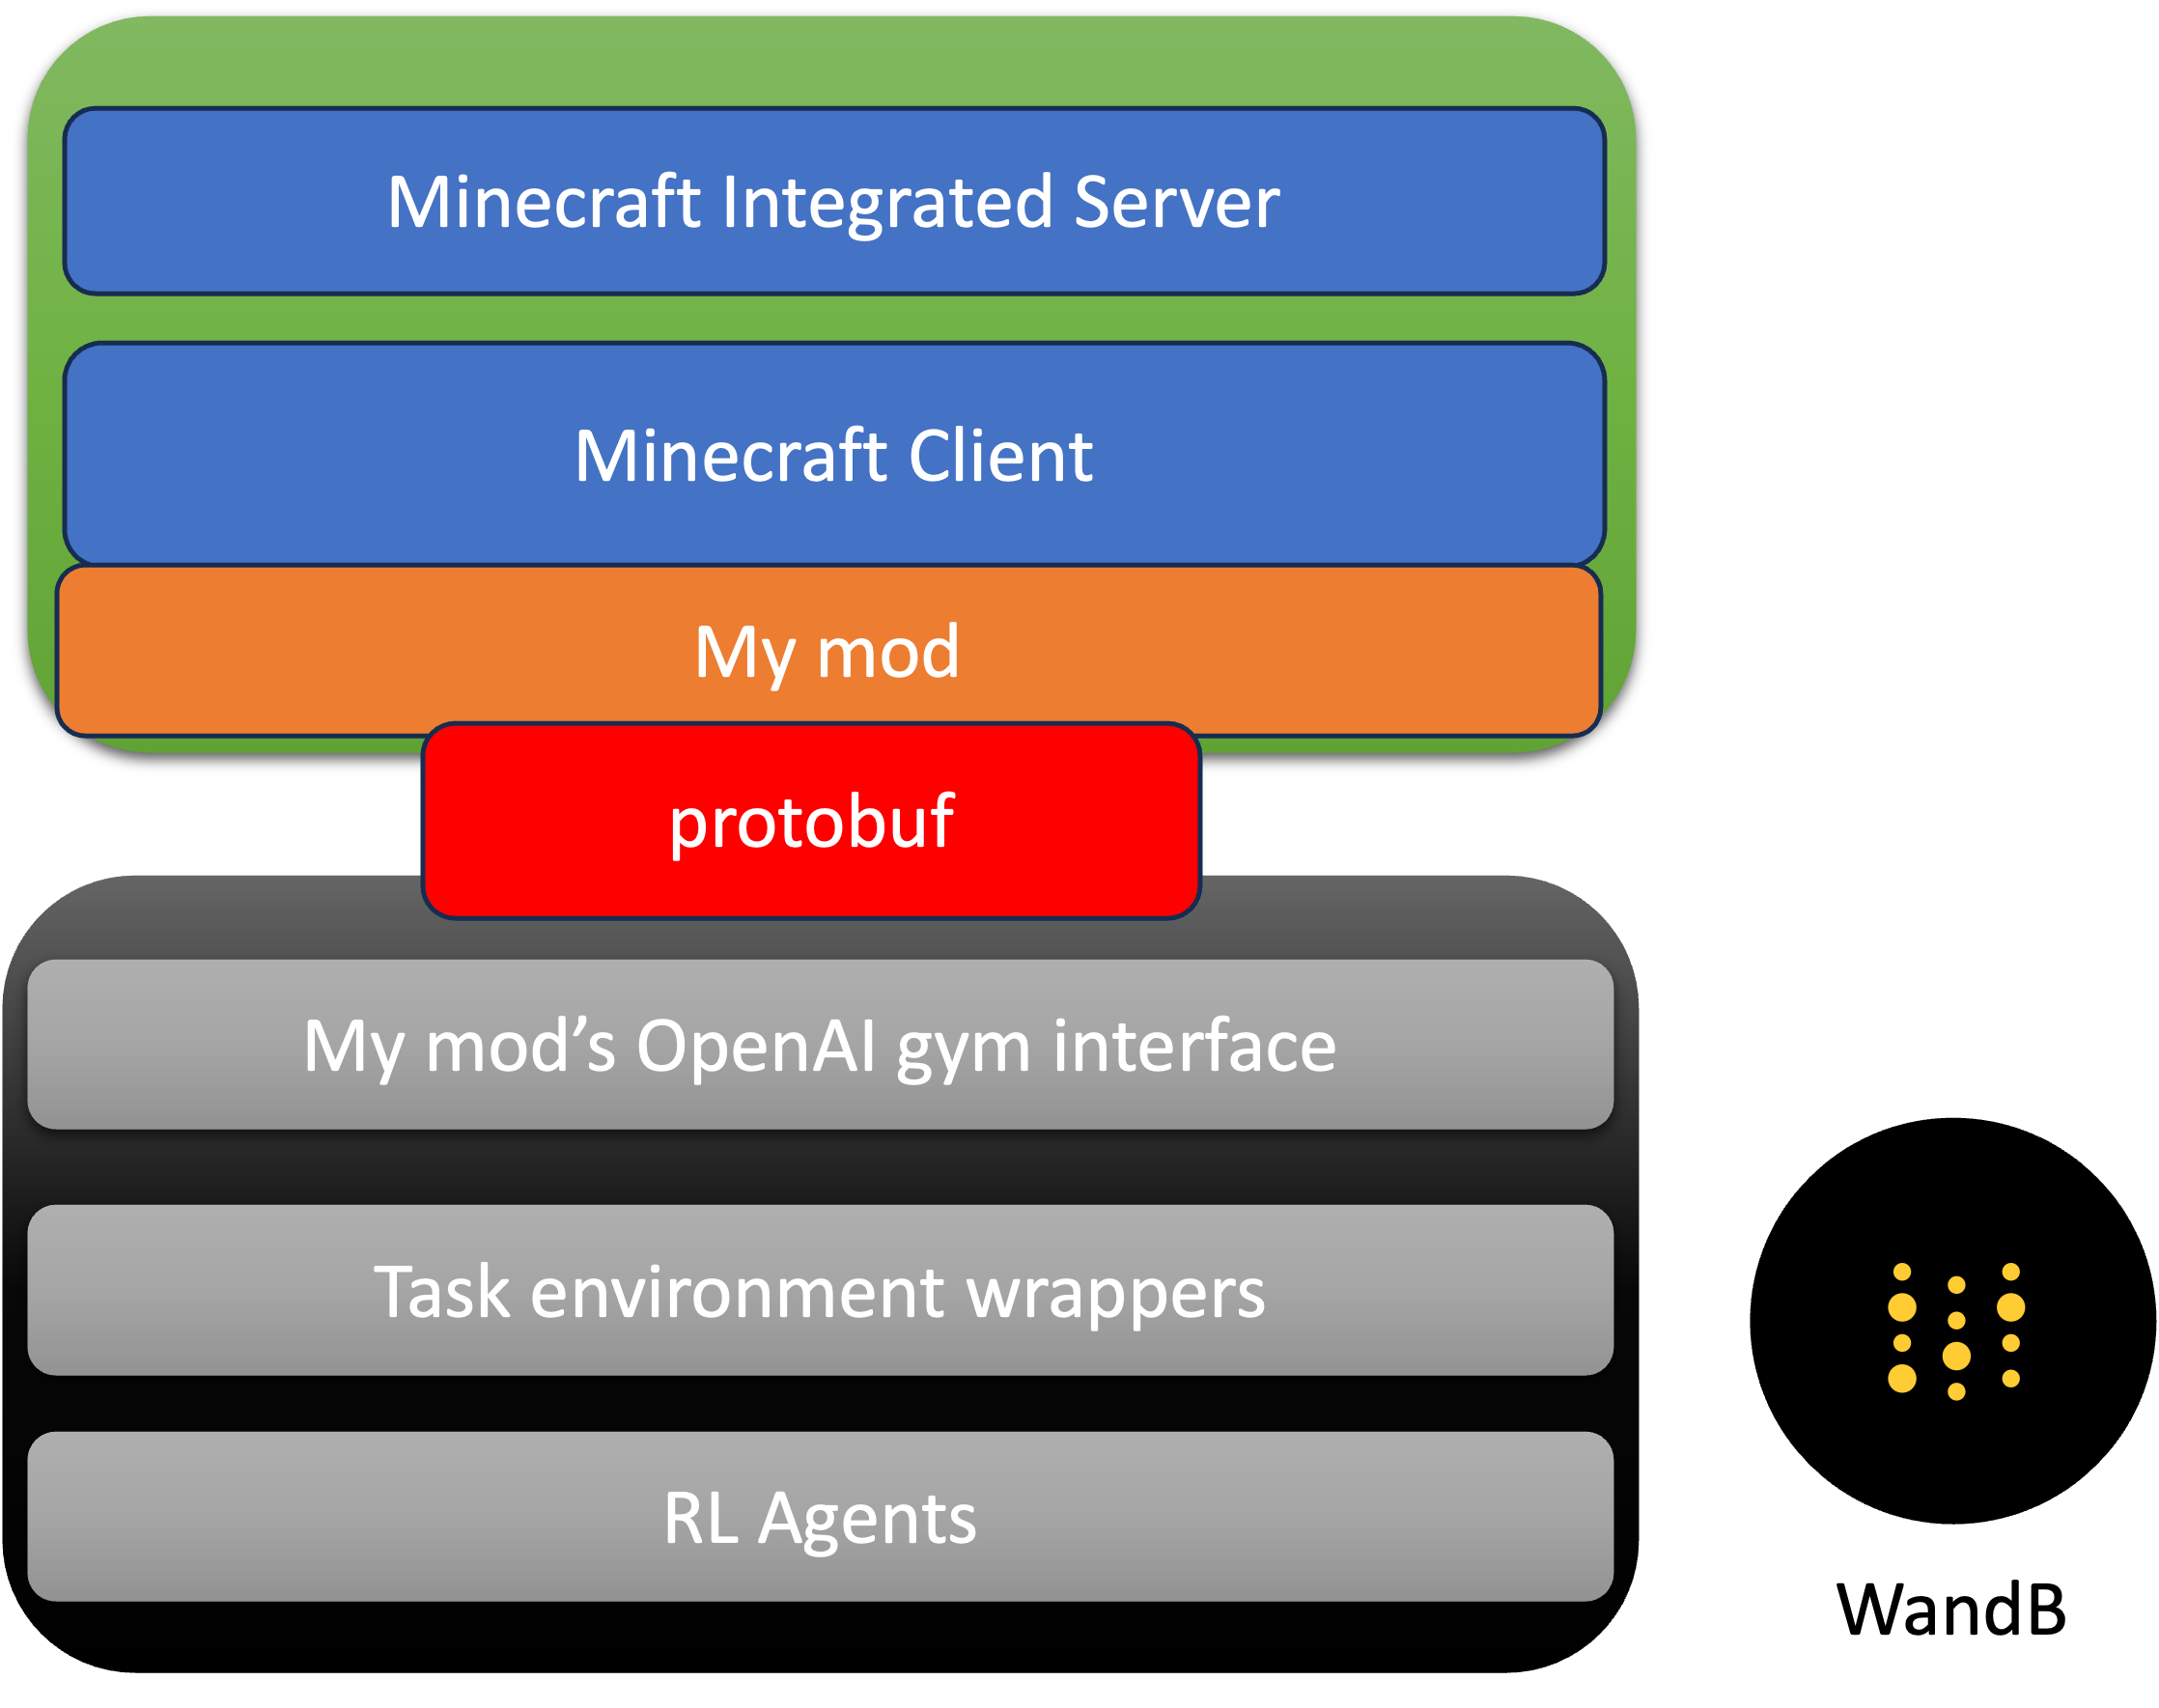
\includegraphics[width=0.5\textwidth]{environment.png}
    \caption{우리 연구에서 개발한 강화학습 환경의 구조를 나타낸 그림이다.}
    \label{fig:environment}
\end{figure}

표 \ref{tab:observation_space}에는 이 환경에서 제공하는 관측 공간 항목들을 소개한다. 이 관측 공간 항목에서, 이 논문에서 소리 정보를 이용하기 위해 활용한 SoundEntry에 대한 상세 정보도 표 \ref{tab:sound_entry}에 소개한다. 또한 표 \ref{tab:initial_environment}에는 이 환경에서 초기에 설정할 수 있는 환경 항목들을 소개한다.

\begin{table}
    \centering
    \renewcommand{\arraystretch}{1.5} % Adjust the line height here
\begin{tabular}{|c|c|c|}
    \hline
    \textbf{필드 이름} & \textbf{타입} & \textbf{설명} \\
    \hline
    image & bytes & 에이전트가 보는 화면 \\
    \hline
    x & double & 에이전트의 X 좌표 \\
    \hline
    y & double & 에이전트의 Y 좌표 (연직 방향) \\
    \hline
    z & double & 에이전트의 Z 좌표 \\
    \hline
    yaw & double & 에이전트가 바라보는 Yaw 각 \\
    \hline
    pitch & double & 에이전트가 바라보는 Pitch 각 \\
    \hline
    health & double & 에이전트의 체력 \\
    \hline
    food\_level & double & 에이전트의 허기  \\
    \hline
    saturation\_level & double & 에이전트의 포만감 \\
    \hline
    is\_dead & bool & 에이전트의 사망 여부 \\
    \hline
    inventory & repeated ItemStack & 에이전트가 소지한 아이템 \\
    \hline
    raycast\_result & HitResult & 에이전트 시선 광선 투사 결과값 \\
    \hline
    sound\_subtitles & repeated SoundEntry & 에이전트 주변에 발생한 소리 이벤트 \\
    \hline
    status\_effects & repeated StatusEffect & 에이전트가 영향받고 있는 상태 효과 \\
    \hline
    killed\_statistics & \texttt{map<string, int32>} & 에이전트가 처치한 몹의 통계 \\
    \hline
    mined\_statistics & \texttt{map<string, int32>} & 에이전트가 채굴한 블록의 통계 \\
    \hline
    misc\_statistics & \texttt{map<string, int32>} & 낚시한 물고기 수, 총 걸음 수 등 기타 통계 \\
    \hline
    visible\_entities & repeated EntityInfo & 현재 에이전트에 보이는 몹의 배열 \\
    \hline
    surrounding\_entities & \texttt{map<int32, EntitiesWithinDistance>} & 에이전트로부터 일정 거리 이내의 몹의 배열 \\
    \hline
\end{tabular}
\caption{환경에서 제공하는 관측 공간 예시}
\label{tab:observation_space}
\end{table}

\begin{table}
    \renewcommand{\arraystretch}{1.5} % Adjust the line height here
    \centering
    \begin{tabular}{|c|c|c|}
      \hline
      \textbf{필드 이름} & \textbf{타입} & \textbf{설명} \\
      \hline
      translate\_key & string & 해당 소리의 종류를 나타내는 고유한 텍스트 \\\hline
      age & int64 & 해당 소리가 발생하고 경과된 틱 수 \\\hline
      x & double & 소리가 발생한 X 좌표 \\\hline
      y & double & 소리가 발생한 Y 좌표 \\\hline
      z & double & 소리가 발생한 Z 좌표 \\
      \hline
    \end{tabular}
    \caption{SoundEntry 모델}
    \label{tab:sound_entry}
\end{table}

\begin{table}
    \renewcommand{\arraystretch}{1.5} % Adjust the line height here
    \centering
    \begin{tabular}{|c|c|c|}
      \hline
      \textbf{필드 이름} & \textbf{타입} & \textbf{설명} \\
      \hline
      initialInventoryCommands & \texttt{repeated string} & 초기에 에이전트에게 제공할 아이템 \\\hline
      initialPosition & \texttt{repeated int32} & 에이전트의 초기 위치. X Y Z yaw pitch 순서이다. \\\hline
      initialMobsCommands & \texttt{repeated string} & 초기에 환경에 생성할 몹 \\\hline
      imageSizeX & \texttt{int32} & 에이전트에게 제공할 화면의 가로 길이 \\\hline
      imageSizeY & \texttt{int32} & 에이전트에게 제공할 화면의 세로 길이 \\\hline
      seed & \texttt{int64} & 세계를 생성할 때의 시드 \\\hline
      allowMobSpawn & \texttt{bool} & 시뮬레이션 도중 몹이 생성될 수 있는지를 제어 \\\hline
      alwaysNight & \texttt{bool} & 시뮬레이션 환경이 항상 밤이어야 하는지를 제어 \\\hline
      alwaysDay & \texttt{bool} & 시뮬레이션 환경이 항상 낮이어야 하는지를 제어 \\\hline
      initialWeather & \texttt{string} & 초기 날씨 상태 \\\hline
      isWorldFlat & \texttt{bool} & 세계가 완전한 평지인지를 제어 \\\hline
      visibleSizeX & \texttt{int32} & 실제 보이는 화면의 가로 크기 \\\hline
      visibleSizeY & \texttt{int32} & 실제 보이는 화면의 세로 크기 \\\hline
      initialExtraCommands & \texttt{repeated string} & 초기화 후 실행할 추가 명령어 \\\hline
      killedStatKeys & \texttt{repeated string} & 에이전트가 처치한 몹의 통계 요청 키 \\\hline
      minedStatKeys & \texttt{repeated string} & 에이전트가 채굴한 블록의 통계 요청 키  \\\hline
      miscStatKeys & \texttt{repeated string} & 그 외 에이전트의 통계 키 \\\hline
      initialBlockStates & \texttt{repeated BlockState} & 초기에 설치할 블록의 배열  \\\hline
      surroundingEntityDistances & \texttt{repeated int32} & 스캔할 주변 몹들의 거리 범위 \\\hline
      hudHidden & \texttt{bool} & HUD의 숨김 여부 제어 \\
      \hline
    \end{tabular}
    \caption{환경 초기화에 사용할 수 있는 옵션들}
    \label{tab:initial_environment}
  \end{table}


\section{구현 상세}
이 절에서는 이 강화학습 환경을 만들 때 생겼던 문제와 이것을 해결하기 위해 사용한 방법들을 소개한다.
\subsection{플레이어 제어}
마인크래프트의 키보드 입력 제어 클래스는 매 틱마다 특정 입력 키들이 눌려 있는지 검사하여 플레이어의 이동 속도를 제어한다. 우리 환경의 경우 실제 사람이 키보드를 누르지 않고 소프트웨어를 이용하여 입력을 제어하므로 이 행동을 그대로 유지하기는 애로사항이 있다. 따라서 Java Mixin을 활용하여 해당 부분을 덮어썼다. 이를 통해 실제 명령을 받고 해석하는 부분에서는 단순하게 변수를 토글하기만 하면 되도록 하였다.

\subsection{화면 관측}
현재 플레이하고 있는 게임 화면을 얻어오기 위해서 마인크래프트에서 기본으로 제공하는 스크린샷 기능을 이용하였다. 스크린샷을 찍을때 호출되는 부분을 응용하여 매 틱 화면을 캡처하고, 이것을 rgb 이미지로 변환하고, 초기에 입력받은 해상도로 리사이징하여 관측 공간 데이터로 제공한다. 이 논문에서는 114 $\times$ 64의 해상도로 실험을 진행하였다.

\subsection{소리 관측}
이번 환경의 핵심인 소리 정보를 제공하기 위하여, 마인크래프트에서 제공하는 접근성 기능인 소리 자막 기능을 활용하였다. 소리 자막 기능을 제공하기 위해 존재하는 소리 이벤트 콜백을 생성 후 등록하여, 게임에서 시뮬레이션 도중 발생하는 소리 이벤트들을 저장한다. 이후 해당 소리 이벤트 정보들은 에이전트에 관측 공간 정보를 제공할 때 같이 제공하였다. 60틱의 시간이 지나면 해당 소리 데이터를 삭제하여 오래된 소리 발생 정보가 남아있지 않도록 하였다.

\subsection{초기화 명령어 실행 후 결과 확인}
실험의 자유도를 위하여 환경 초기화 시 임의의 마인크래프트 명령어를 실행할 수 있게 하였다. 이 명령어의 실행이 완전히 완료된 후부터 에피소드가 진행되는데, 이를 위하여 명령어 실행 후 채팅 메시지가 발생하는 현상을 이용하였다. 일련의 명령어의 끝에 종료 메시지를 출력하는 명령어를 추가하고, 이 종료 메시지가 출력되었을 때 화면의 모든 채팅 메시지를 삭제한 후, 에이전트에게 제어권을 넘겨주었다.

\subsection{청소년 보호 기능 해제}
마인크래프트는 기본적으로 대한민국에서 청소년 보호 기능이 활성화되어 있어, 1시간 이상 게임을 플레이하면 자동으로 지나친 게임 이용에 대해 경고하는 메시지가 출력된다. 비전을 이용하는 에이전트의 경우, 이 메시지에 의해 학습의 신뢰도를 떨어뜨릴 수 있다. 이를 해제하기 위하여, Mixin을 이용하여 해당 기능을 해제하였다.


\chapter{다양한 환경들에서의 실험}
이전 장에서 설명한 강화학습 환경을 이용하여 다양한 실험들을 진행하였다. 이 다양한 환경들에서 소리만 이용할 때, rgb 화면만 이용할 때, 그리고 소리와 rgb 화면을 모두 활용하는 바이모달 에이전트를 사용할 때 실험을 하여 성능을 비교하였다. 이러한 실험을 진행하는데 사용한 python 코드는 GitHub 저장소\footnote{\url{https://github.com/KYHSGeekCode/MinecraftRL}} 에서 확인할 수 있다.

\section{실험 환경}
이 논문에 활용한 실험 환경은 총 4가지\footnote{\url{https://github.com/KYHSGeekCode/MinecraftRL/tree/main/final_experiments}에서 건물 탐험 등 더 다양한 환경들을 찾아볼 수 있다.}이다. 이 논문에서 허스크란 플레이어를 쫓아 공격하는 마인크래프트의 몬스터로서, 비슷한 행동을 보이는 좀비의 변종이다. 실험을 진행하는 낮에 태양빛에 면역이기 때문에 이번 실험에 선택되었다. 그림에서 허스크가 삽을 들고 있는 것을 알 수 있는데, 허스크의 공격력을 조정하여 플레이어가 3$\sim$4회 피격 시 사망하여 시뮬레이션을 종료할 수 있게 하였다. 실험 환경은 다음과 같다.
\begin{enumerate}
    \item (허스크) 무한한 평면 위에서, 무작위로 5 $\sim$ 10블록 떨어진 곳에 생성되는 허스크 회피.
    \item (허스크 2) 무한한 평면 위에서, 무작위로 5 $\sim$ 10블록 떨어진 곳에 생성되는 4마리의 허스크 회피.
    \item (지형-허스크) 나무와 풀, 꽃, 언덕이 존재하는 지형 위에서, 무작위로 5$\sim$10블록 떨어진 곳에서 생성되는 허스크 회피
    \item (동물) $11 \times 11$ 크기의 목장에서 무작위로 4개 중 3곳에 갇혀 생성되는 각 7마리의 동물들 중 지정된 동물 찾아가기.
\end{enumerate}

이 환경들에 해당하는 화면들을 그림 \ref{fig:environment_images}에 나타내었다.

"허스크 2" 환경의 경우, 마인크래프트 세계를 생성할 때 입력하는 시드를 \lstinline{3788863154090864390}으로 고정하였다. 마인크래프트의 시드는 세계 생성 시 지형 및 구조물의 위치를 결정한다. 따라서 시드가 같으면 다양한 에이전트를 항상 같은 지형에서 테스트하여 성능을 비교할 수 있다. 해당 시드로 생성한 세계에는 완만한 언덕이 있어 지형과 장애물이 있는 곳에서 허스크를 회피하는 실험을 진행하기 좋다고 생각하여 해당 시드를 이용하였다.

\begin{figure}[htp]
    \centering
    \begin{tabular}{cc}
        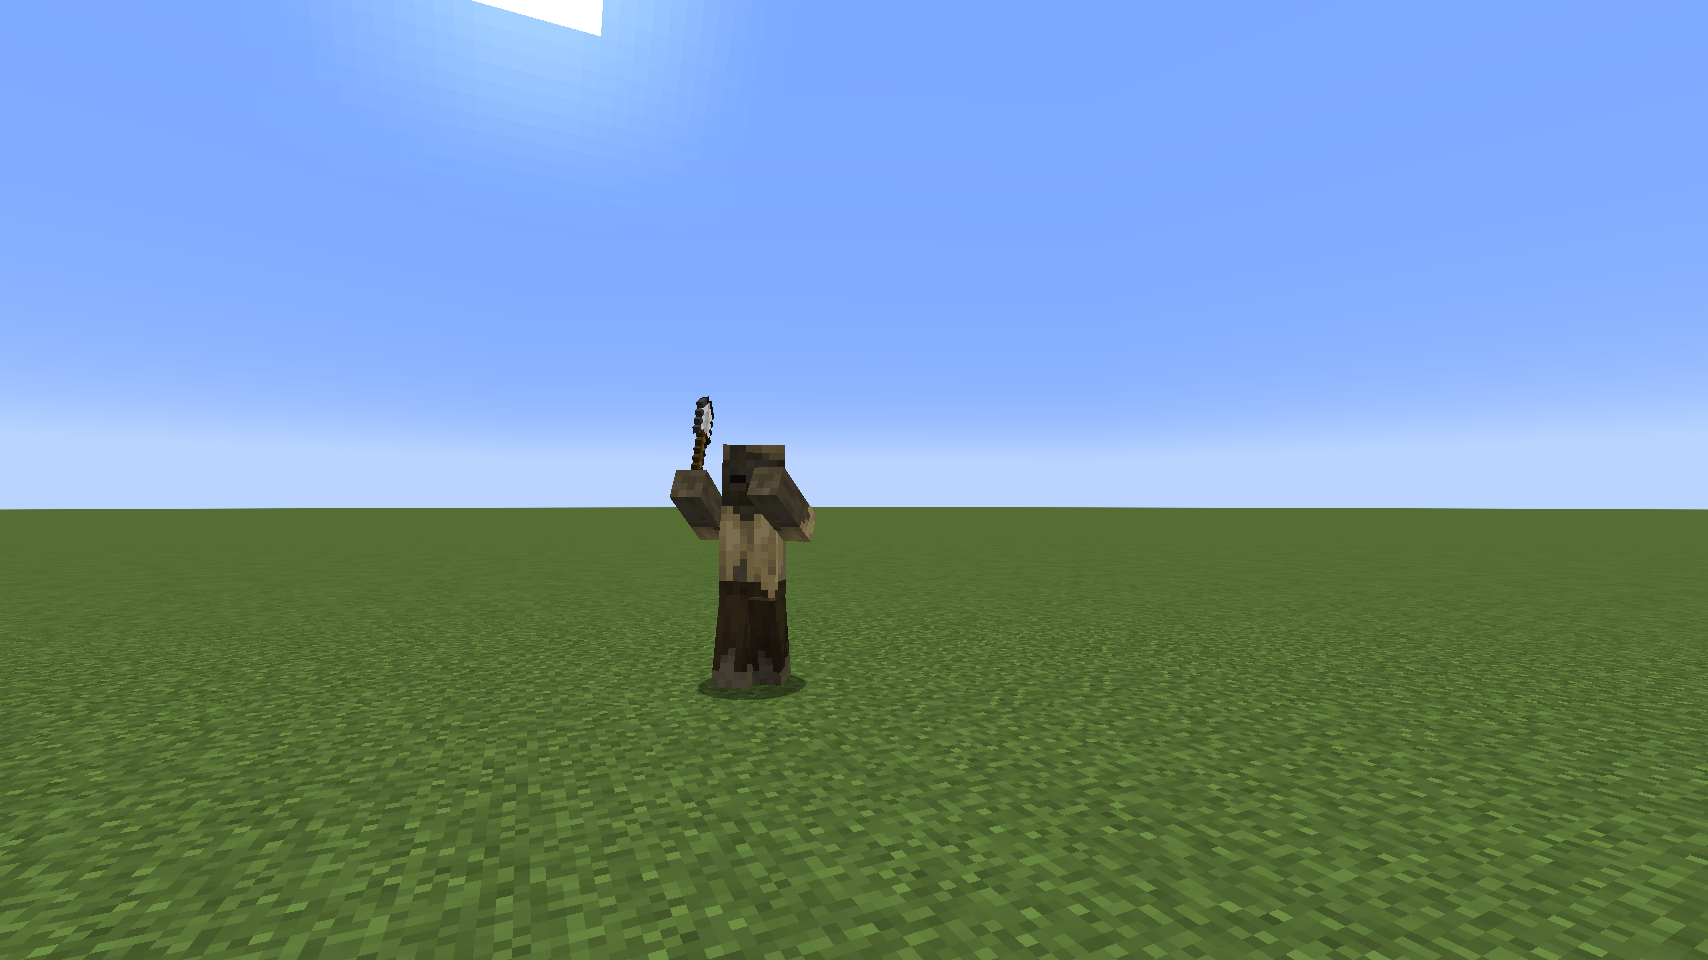
\includegraphics[width=0.5\textwidth]{env_husk} & 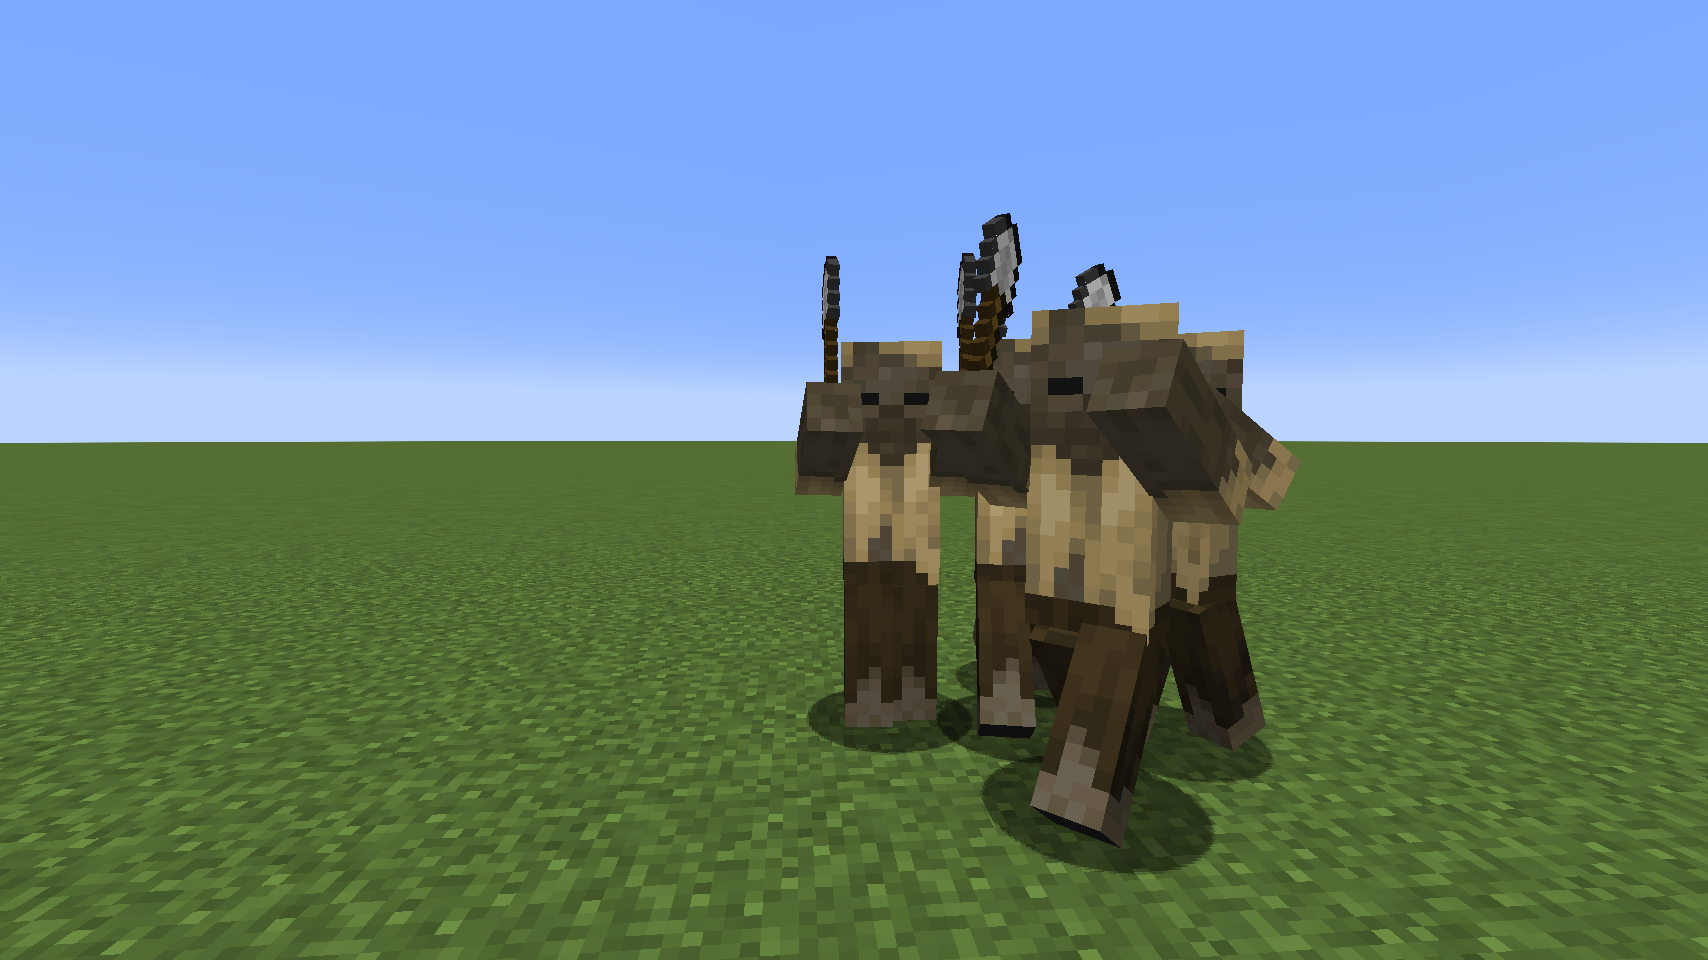
\includegraphics[width=0.5\textwidth]{env_husks} \\
        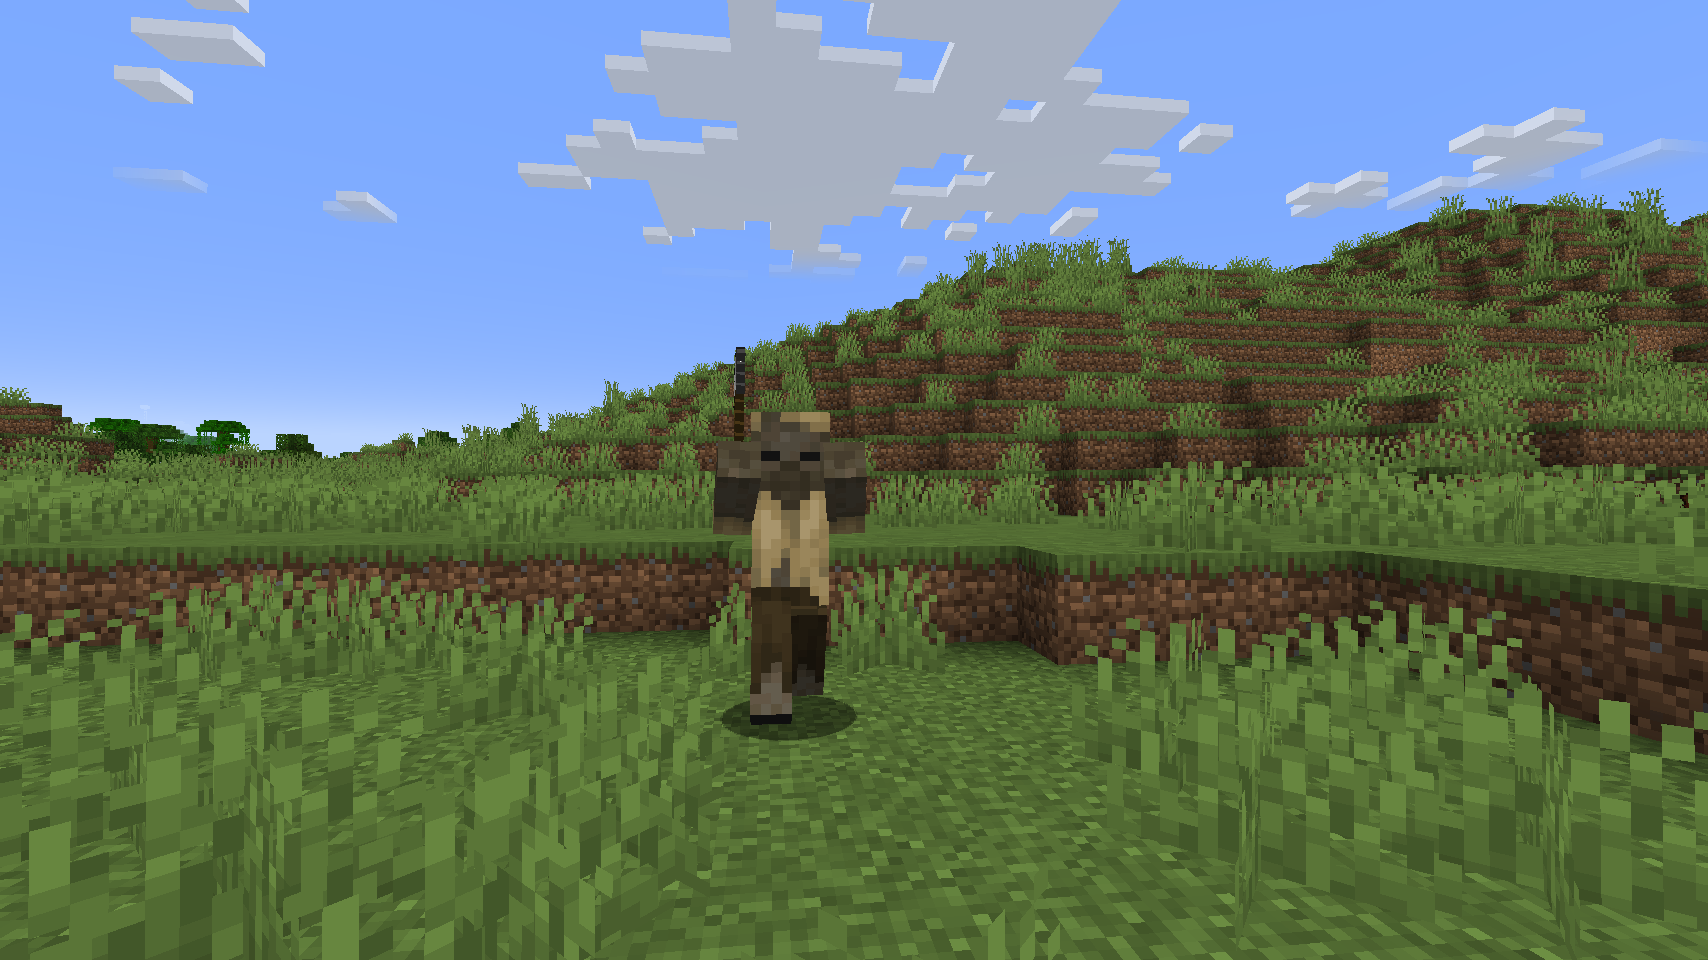
\includegraphics[width=0.5\textwidth]{env_terrain_husk} & 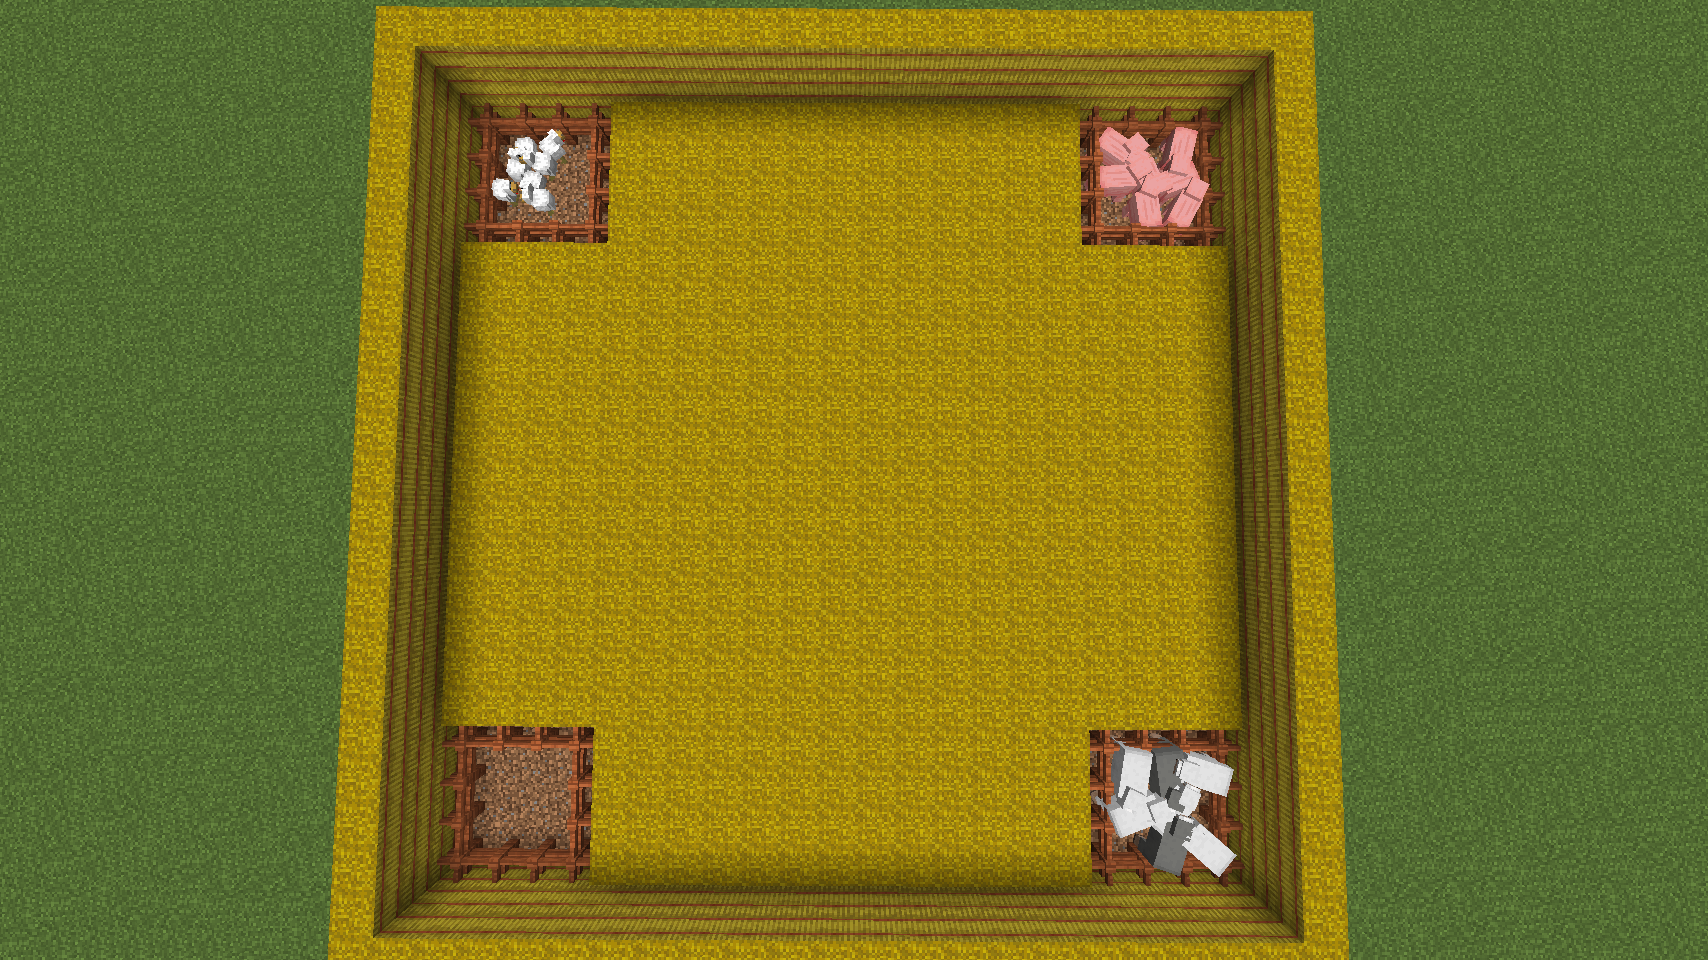
\includegraphics[width=0.5\textwidth]{env_animal} \\
    \end{tabular}
    \caption{에이전트가 마주하는 환경들을 나타내는 그림. 왼쪽 위에서부터 허스크, 허스크 2, 지형-허스크, 동물 환경이며, 동물 환경의 경우 이해를 돕기 위해 위에서 내려다본 모습을 나타내었다. 허스크 2의 경우 허스크 여러 마리가 다양한 좌표에서 동시 생성된다.}
    \label{fig:environment_images}
\end{figure}


허스크를 회피하는 태스크(허스크, 허스크 2, 지형-허스크)의 경우, 다음과 같은 보상을 제공하였다.
\begin{itemize}
    \item 허스크에게 공격받아 체력이 감소할 경우, $-0.1$
    \item 허스크의 공격으로 사망할 경우, $-1$ 제공 후 시뮬레이션 종료
    \item 그렇지 않을 경우 매 틱마다 $0.5$
\end{itemize}
동물을 찾아가는 태스크의 경우, 다음과 같은 보상을 제공하였다.
\begin{itemize}
    \item 주변 2m 이내에 지정한 동물이 전부 존재할 경우, 1 제공 후 시뮬레이션 종료
    \item 이외의 경우, 0
\end{itemize}

이 환경들의 특징은 부분 관측 가능한 마르코프 프로세스(POMDP) 환경이라는 것이다. 에이전트가 받는 입력인 소리나 화면 정보는, 현재 해당 에이전트가 처한 환경을 전부 표현할 수 없다. 이런 환경에서는 에이전트가 보는 최신 화면만으로는 어떤 두 상황이 같은 상황인지 확신할 수가 없으며, 이에 따라 그 화면에서 최적의 행동이 상황마다 다를 수 있다는 특징이 있다. 소리 입력의 경우에도 그 자체만으로는 항상 발생하지는 않고 일정 주기로 발생하는 특징이 있는데, 이에 따라 소리가 나지 않더라도 주변에 허스크가 있을 수 있다는 특징이 있다.

이러한 환경에서의 강화 학습 문제를 해결하기 위해서 DRQN (Deep Recurrent Q Network) 등과 같은 아키텍처가 제안되었다. \cite{POMDP} 이번 논문에서는 같은 문제를 해결하기 위해 여러 입력을 활용하는 바이모달 모델을 이용하는 실험을 진행한다.

동물을 찾아가는 태스크의 경우, 최종 도착 여부에 따른 0 또는 1의 보상만 주어지기 때문에 보상이 희박하다는 sparse reward 특징이 있다. 이러한 sparse reward 환경에서 다양한 모달리티의 에이전트가 보이는 성능을 비전 기반 에이전트가 보이는 성능과 비교해볼 것이다.

\section{행동 공간}
에이전트가 각 환경에서 선택할 수 있는 행동은 다음과 같다.
\begin{itemize}
    \item (허스크), (허스크 2): 정지, 앞으로 가기, 뒤로 가기, 왼쪽으로 가기, 오른쪽으로 가기, 왼쪽으로 돌기, 오른쪽으로 돌기
    \item (지형-허스크): 정지, 앞으로 가기, 뒤로 가기, 왼쪽으로 가기, 오른쪽으로 가기, 왼쪽으로 돌기, 오른쪽으로 돌기, 점프
    \item (동물): 앞으로 가기, 왼쪽으로 돌기, 오른쪽으로 돌기
\end{itemize}
여기서 왼쪽으로 가기와 오른쪽으로 가기는 플레이어가 바라보는 방향의 왼쪽 $90^\circ$, 오른쪽 $90^\circ$ 방향으로 이동하는 옆걸음질을 뜻한다.

\section{모델}
이 연구에서 사용한 강화학습 모델은 Dueling DQN \cite{DuelingDQN}이다. 주어진 관측 공간에서 특징을 추출하고, 어드밴티지와 현재 상태에 대한 값을 추정하는 상세한 모델 구조를 그림 \ref{fig:models}에 나타내었다. 세 모델은 공통적으로 특징 추출 부분과 Advantage, Value network로 나뉘어 있다.

\begin{figure}[htp]
    \centering
    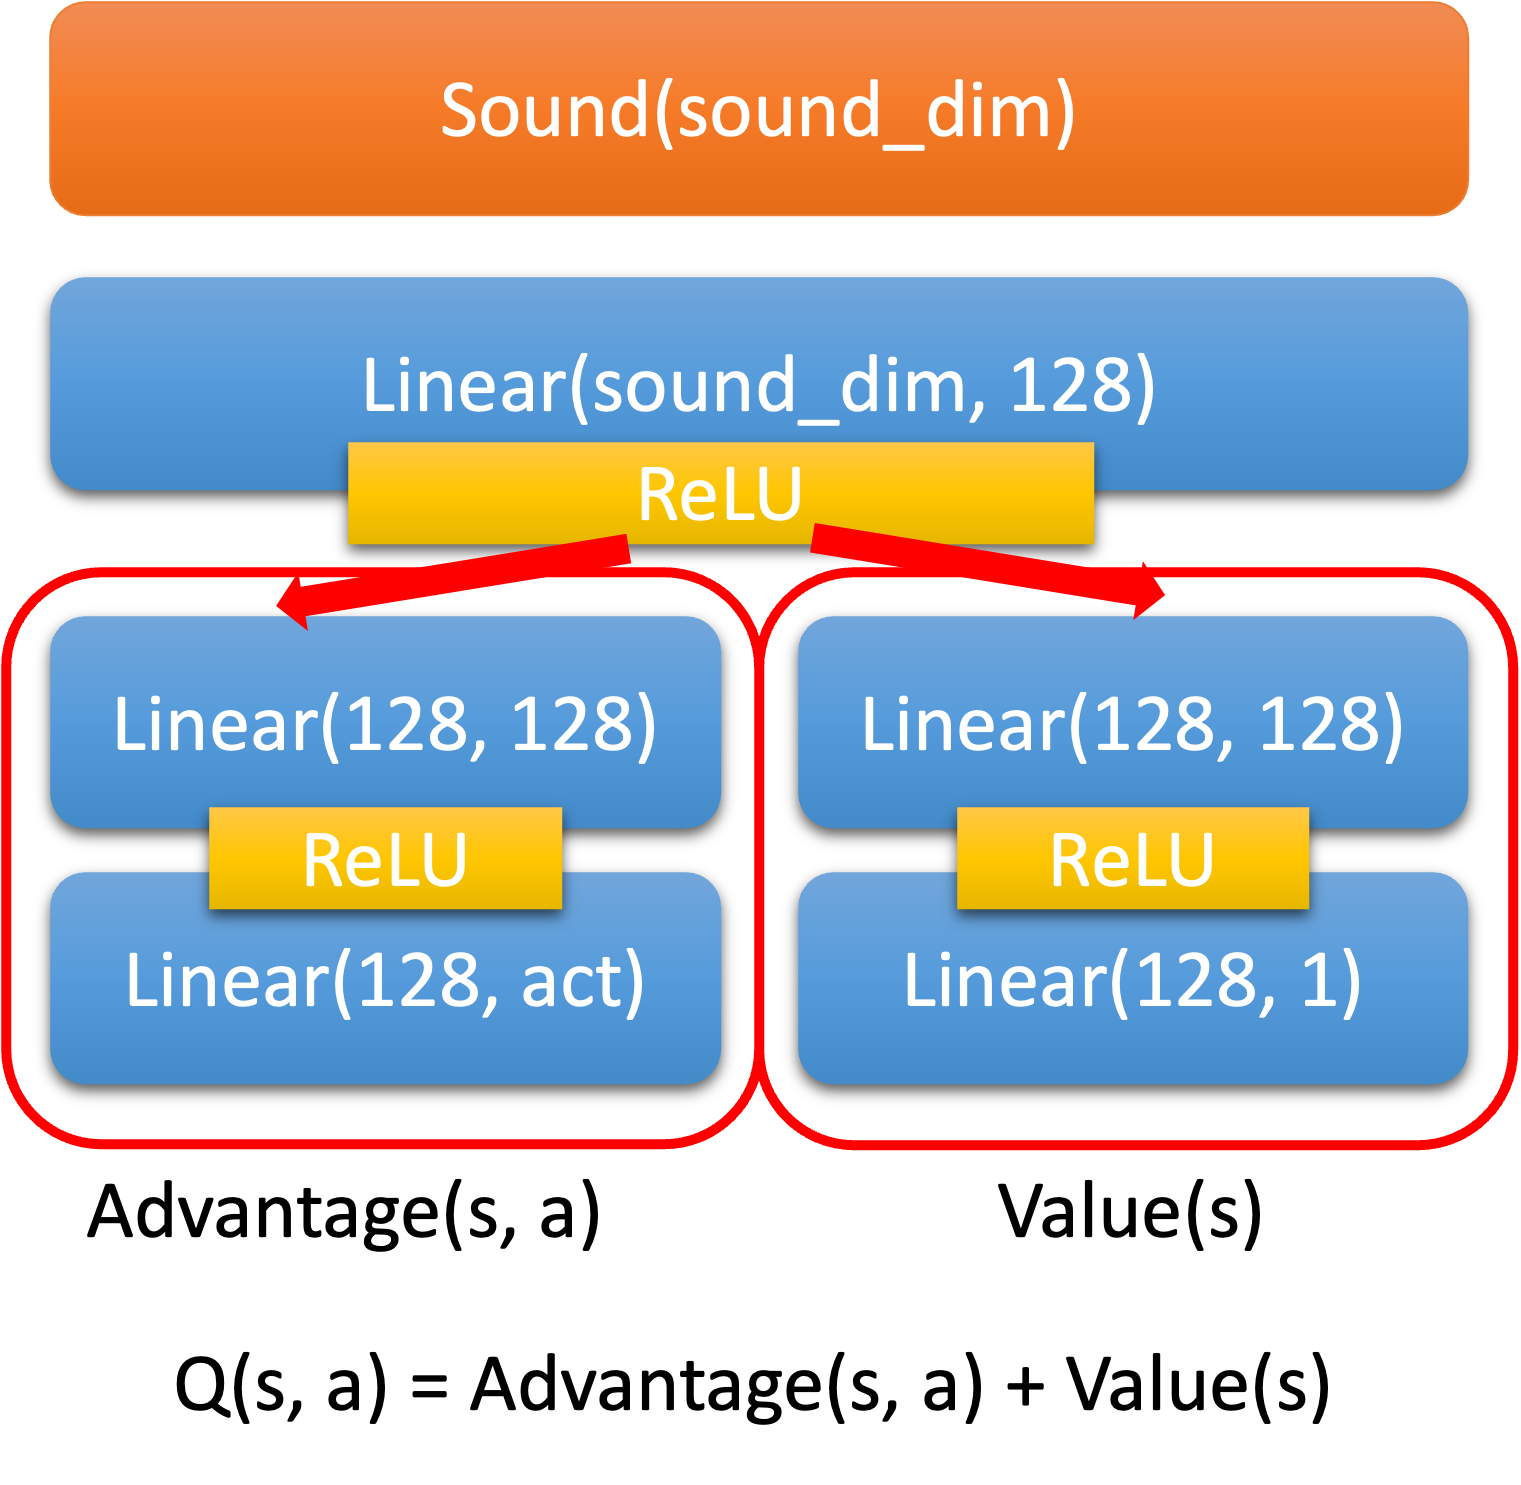
\includegraphics[width=.33\textwidth]{sound_dueling_dqn}\hfill
    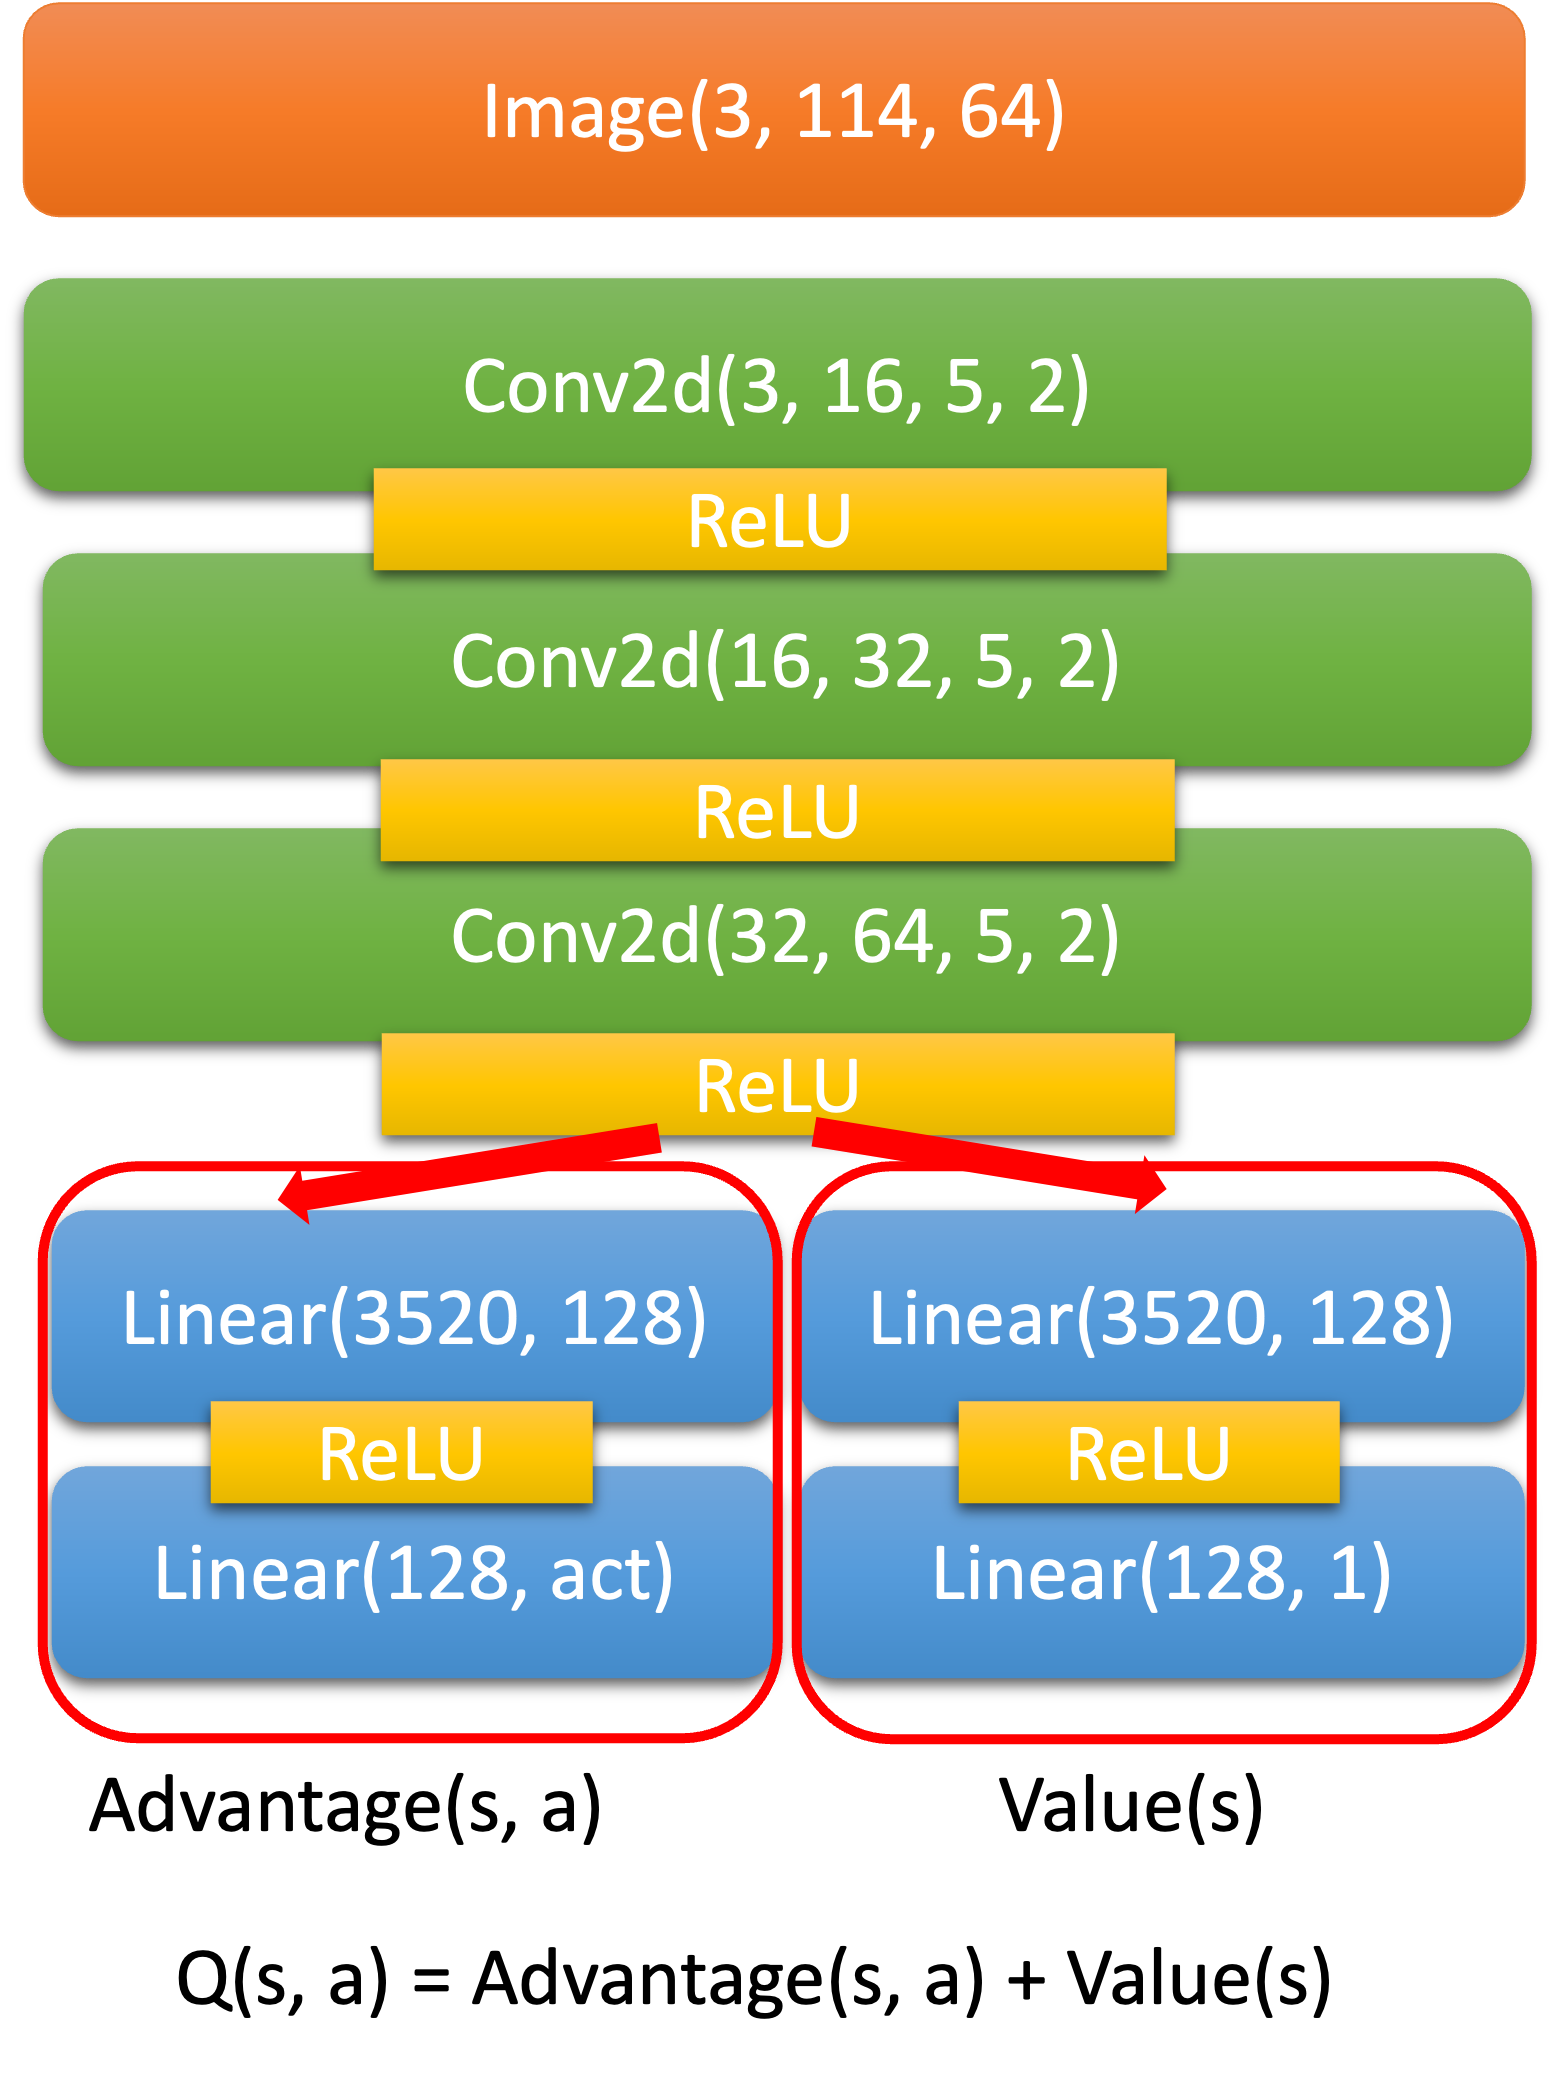
\includegraphics[width=.33\textwidth]{vision_dueling_dqn.png}\hfill
    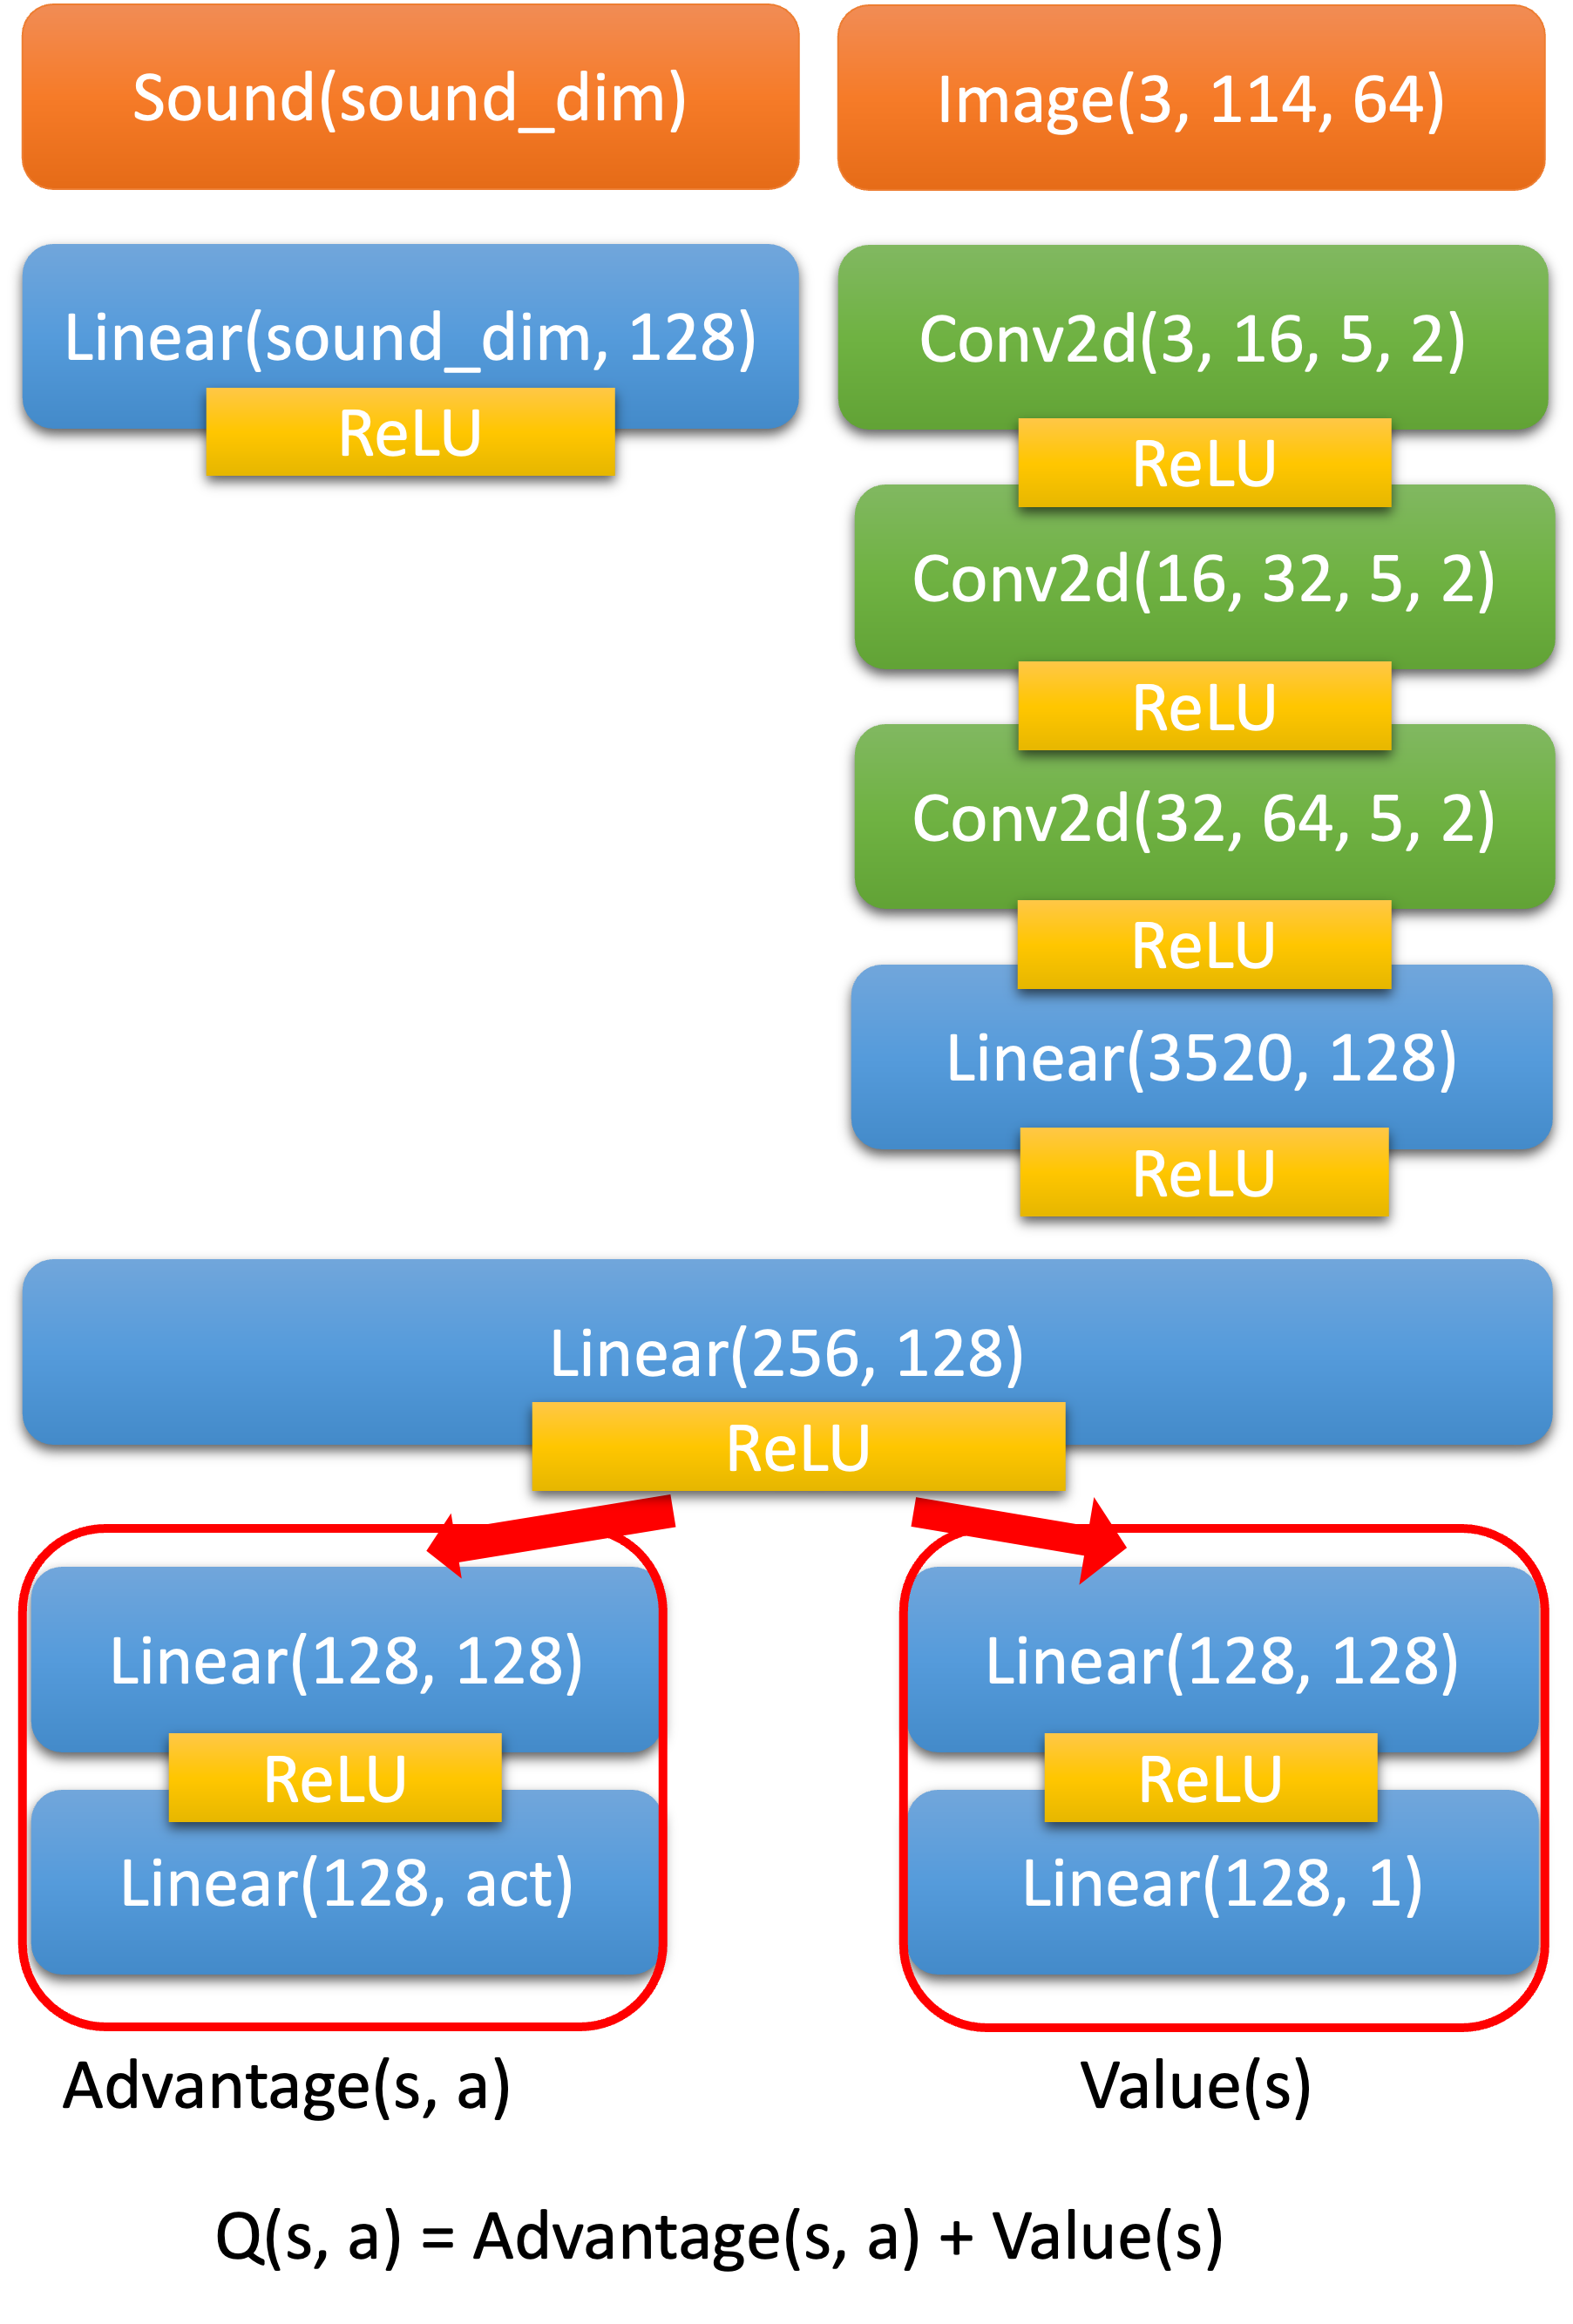
\includegraphics[width=.33\textwidth]{bimodal_dueling_dqn}
    
    \caption{이번 연구에서 활용된 에이전트를 위한 세 가지 모델을 나타낸다. 왼쪽부터 소리 입력을 받는 모델, 화면 입력을 받는 모델, 소리와 화면 입력을 받는 모델이다. 주황색 부분은 입력, 파란색 부분은 Linear 네트워크, 초록색 부분은 Convolutional 네트워크를 나타낸다. ReLU 활성화 함수를 사용하였으며, 입력 컴포넌트의 괄호 안의 숫자는 해당 데이터의 차원을 나타낸다. Linear 네트워크 컴포넌트의 괄호 안의 숫자는 각각 입력 차원과 출력 차원을 나타낸다. Convolutional 네트워크 컴포넌트의 괄호 안의 숫자는 각각 입력 채널 수, 출력 채널 수, 커널 크기, 스트라이드 크기를 나타낸다. 소리와 화면 입력을 받는 모델에서는 Advantage와 Value Network로 데이터를 전달하기 전에 각각의 모드에서 추출된 특징 벡터가 하나로 연결된다.}
    \label{fig:models}
\end{figure}

소리 입력을 받는 모델의 경우, 우선 환경에서는 해당 환경에서 발생할 수 있는 소리마다 1) 평면 태스크의 경우 2차원, 2) 지형이 있는 태스크의 경우 3차원을 할당하여 상대 좌표 dx, dy, dz를 제공하는 벡터를 만들고, 현재 에이전트가 바라보고 있는 수평 방향을 나타내는 yaw값을 cos, sin 값을 취해 제공한다.\cite{Rotation} 또한 플레이어가 대미지를 입는 소리의 경우 항상 플레이어의 위치에서 발생하므로 별도의 2/3차원을 이용하지 않고 0 또는 1로 인코딩하여 제공한다. 따라서 모델이 입력받는 벡터의 차원은 $2$ or $3$ $\times$ (소리의 종류) $ + 3$ 이 된다. 이 벡터를 이용하여 완전연결신경망을 이용하여 특징을 추출한 후, 각각 Advantage network와 Value network에 제공한다. Advantage network는 이 상황에서 action별로 예상되는 advantage를 계산하고, Value network는 이 상황 자체의 가치를 평가한다. 이 둘을 합쳐 Q value를 예상한다.

이미지 입력을 받는 모델의 경우, 환경에서 제공받은 3채널 (r, g, b) $114 \times 64$ 이미지를 3층의 합성곱 신경망에 통과시켜 특징을 추출한다. 그림에 나와 있는 합성곱 신경망의 괄호 안에 쓰여 있는 숫자의 뜻은 (입력 채널 수, 출력 채널 수, 커널 크기, stride)이다. 이후 이렇게 추출된 특징을 이용하여 Advantage와 Value, 최종적으로 Q value를 예상한다.

소리와 이미지를 모두 입력받는 모델의 경우, 환경에서 받은 소리와 이미지 정보의 특징을 각각 추출한 후, 하나의 벡터로 연결하여 Advantage와 Value network의 입력으로 제공한다. 이 신경망을 이용하여 DQN 에이전트들을 생성했다. 리플레이 버퍼를 이용하여 매 상호작용에서 발생한 상태 변화와 보상을 기억하고, 매 1000스텝마다 리플레이 버퍼에서 256개의 샘플을 추출하여 policy q network를 학습시켰다. Epsilon greedy 전략을 사용하여 초기 탐색을 하였으며, warmup 방법을 이용하여 첫 10 에피소드는 리플레이 버퍼를 채우는 데 사용하였다. 이후 임의 행동을 수행할 확률인 epsilon을 1에서 매 에피소드마다 0.99를 곱하여 점점 감소시켜 최종적으로는 0.01로 유지했다.

\section{하이퍼파라미터}
다음과 같은 매개변수를 이용하여 학습을 진행하였다.
\begin{itemize}
    \item batch size: policy network를 학습시킬 때 사용한 배치 사이즈: 256
    \item gamma: 벨만 방정식에서 사용한 감가율: 0.99
    \item learning rate: 학습률 0.00001
    \item update freq: 매 1000 스텝마다 policy network를 학습시켰다.
    \item weight decay: Adam optimizer의 weight decay: 0.00001
    \item buffer size: 리플레이 버퍼의 크기: 1000000
    \item epsilon init: 초기 탐험률 1.0,
    \item epsilon decay: 매 에피소드마다 epsilon에 0.99를 곱해주었다.
    \item epsilon min: 최소 탐험률 0.01
    \item max steps per episode: 허스크 피하기 태스크의 경우 에피소드당 최대 400틱, 동물 찾기 태스크의 경우 에피소드당 최대 600틱이 주어졌다.
\end{itemize}
태스크별 하이퍼파라미터 미세조정은 진행하지 않았다.

\chapter{실험 결과}
아래에 이번에 진행한 여러 실험에서 각 소리, 비전, 멀티모달 에이전트들이 획득한 평균 보상을 나타낸 그래프들을 나타내었다. 가로축은 진행한 에피소드 수이며, 세로축은 각 에이전트가 해당 에피소드에서 획득한 총 보상을 의미한다. 허스크로부터 도망가는 태스크에서 얻을 수 있는 최대 보상은 $400 \times 0.5 = 200 $이고, 동물 찾기 태스크에서 얻을 수 있는 최대 보상은 $1$이다.
\begin{figure}[H]
    \centering
    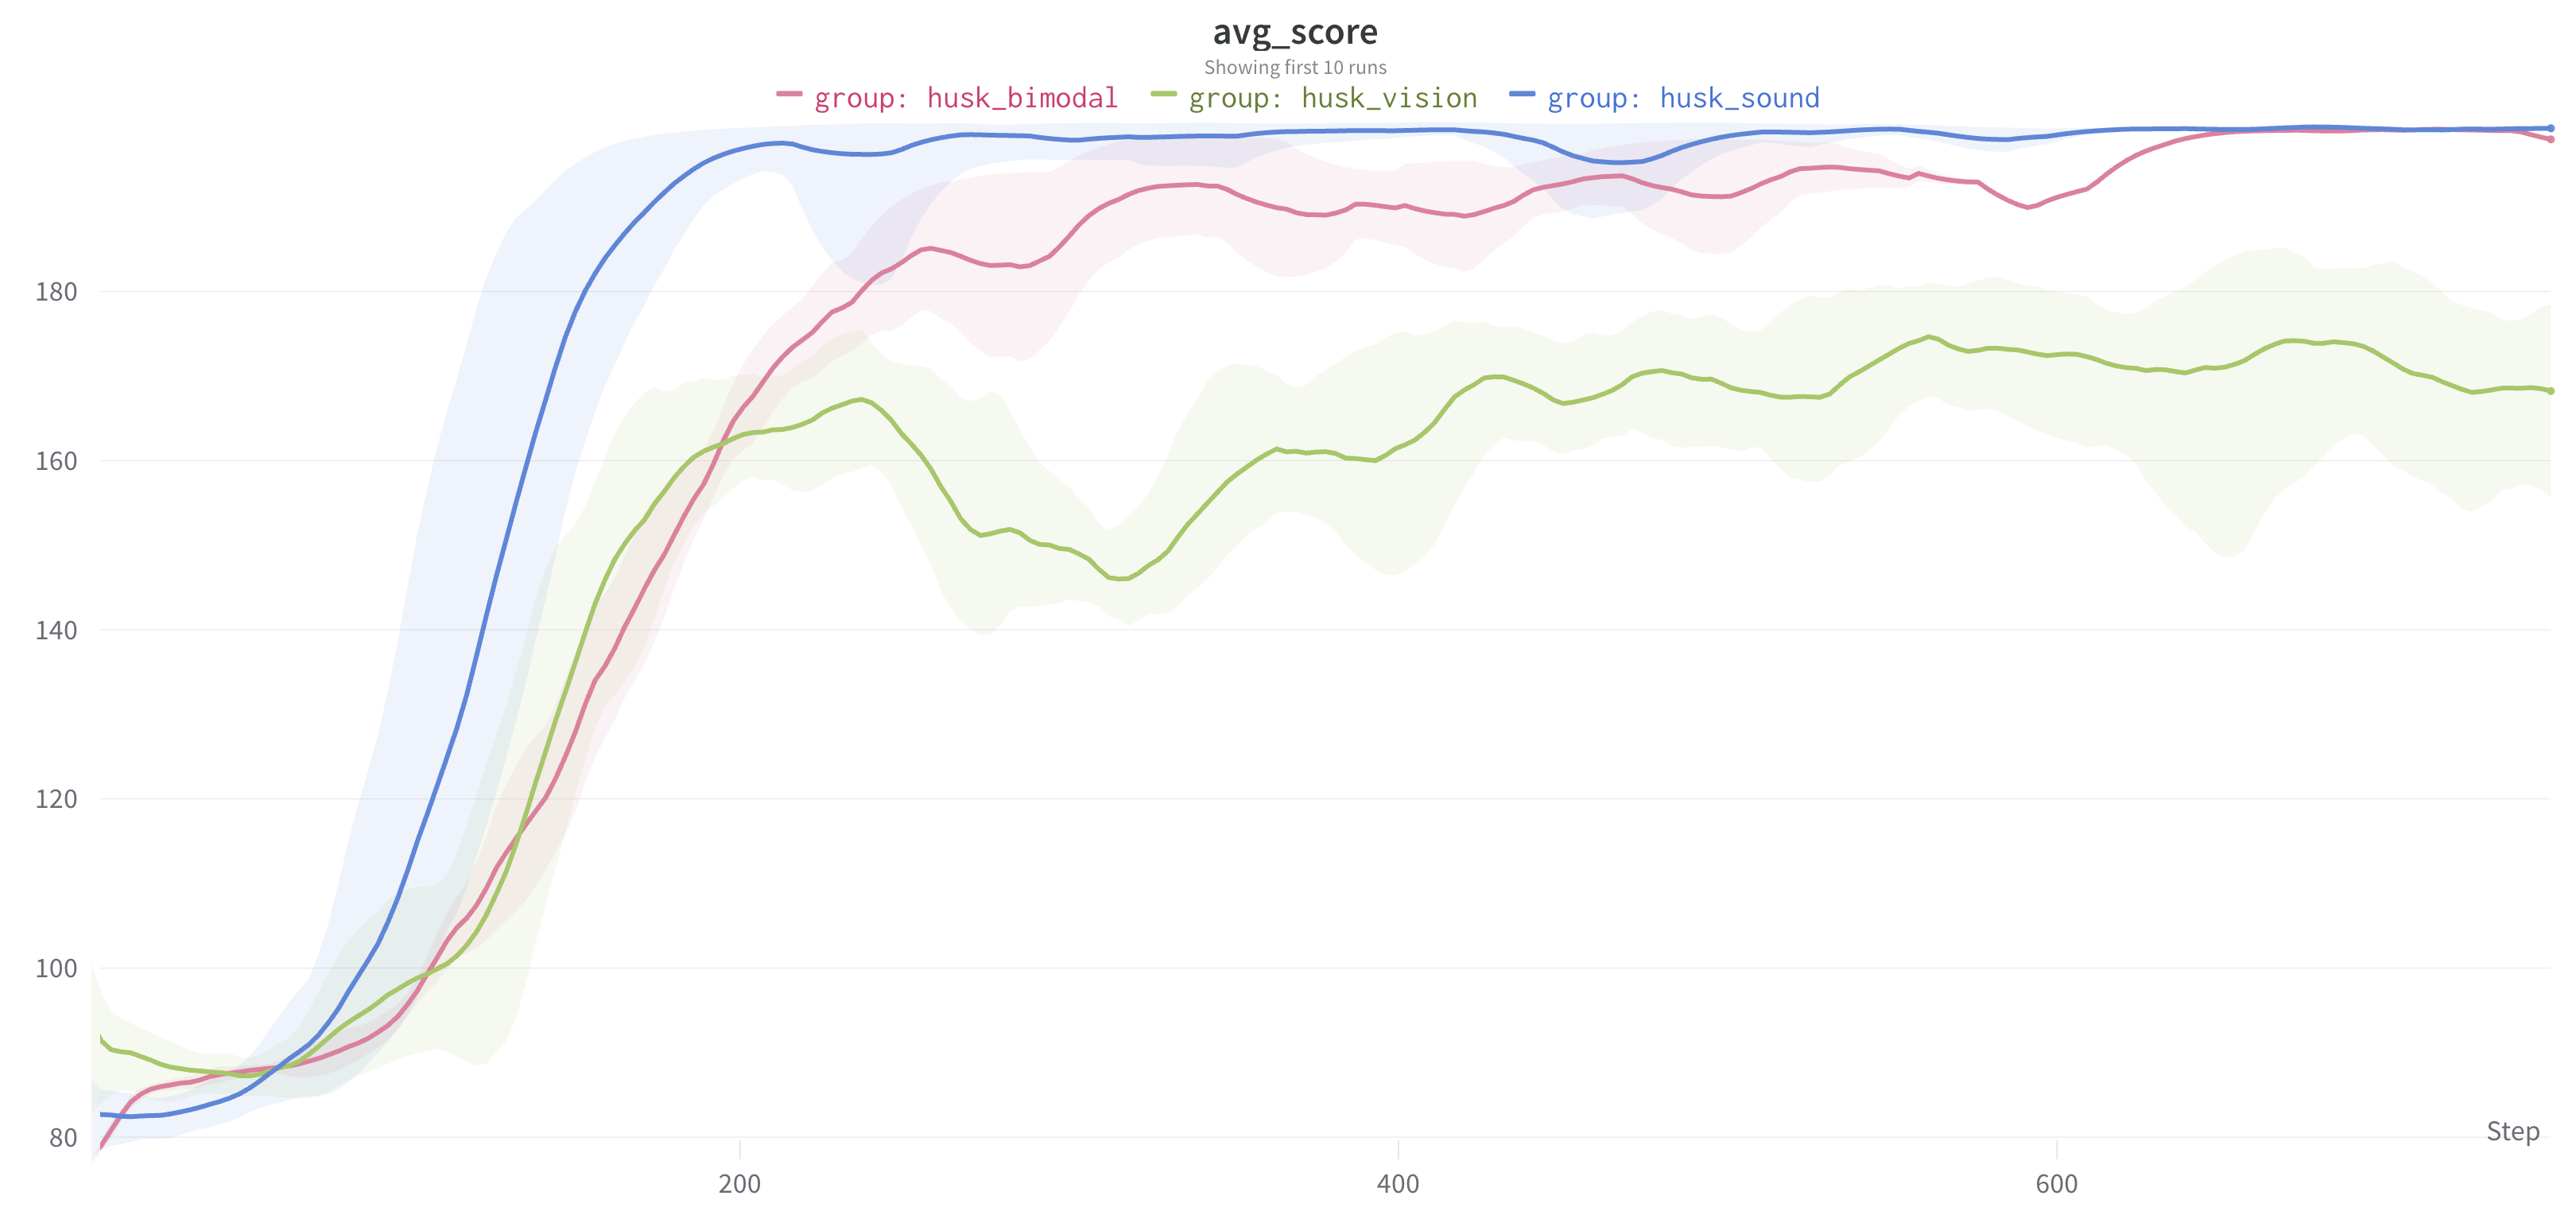
\includegraphics[width=\textwidth]{husk.png}
    \caption{허스크 회피 태스크(허스크 1)에 대한 비전, 소리, 멀티모달 에이전트의 성능을 나타낸 그래프이다.}
    \label{fig:husk}
\end{figure}
그림 \ref{fig:husk}를 보면 \lstinline{husk_vision}으로 나타낸 비전 에이전트도 어느 정도 학습이 이루어진 것을 알 수 있지만, \lstinline{husk_sound}로 나타나는 소리 에이전트와 \lstinline{husk_multimodal}로 나타낸 멀티모달 에이전트가 가장 높은 보상을 얻은 것을 알 수 있다. 또한 멀티모달 에이전트는 증가한 파라미터로 인해 학습이 소리 에이전트에 비해 느려진 것을 확인할 수 있다.

\begin{figure}[H]
    \centering
    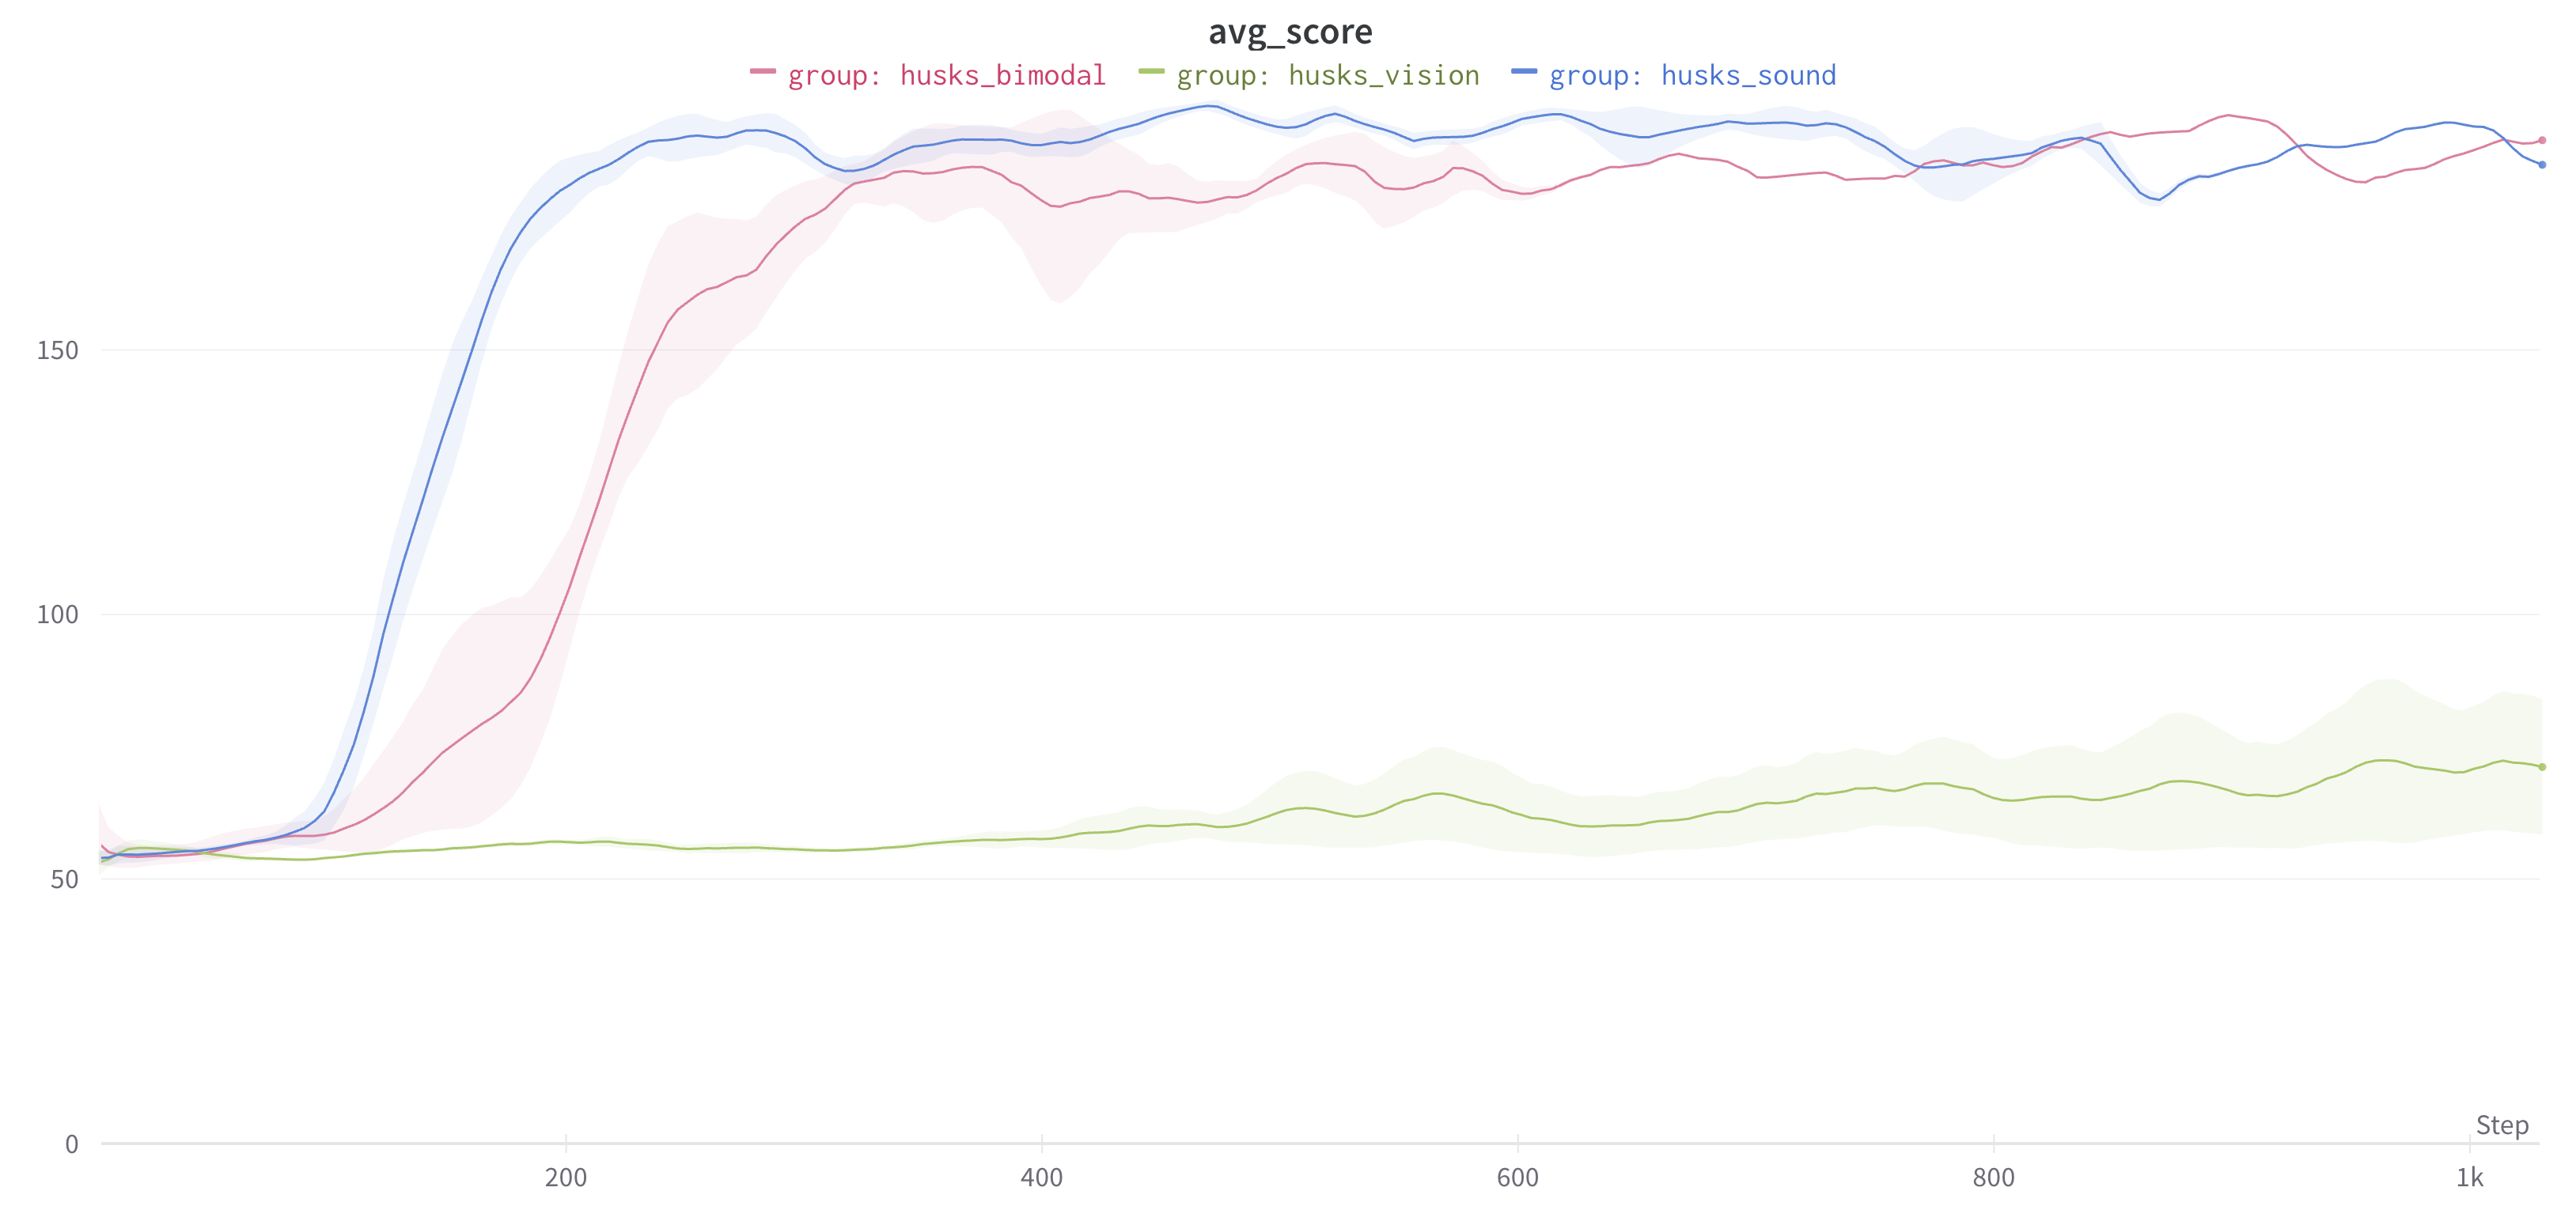
\includegraphics[width=\textwidth]{husks.png}
    \caption{여러 허스크 회피 태스크 (허스크 2)에 대한 비전, 소리, 멀티모달 에이전트의 성능을 나타낸 그래프이다. }
    \label{fig:husks}
\end{figure}
그림 \ref{fig:husks}를 보면 \lstinline{husks_vision}으로 나타낸 비전 에이전트는 거의 상황에 대처하지 못하는 것을 볼 수 있으며, \lstinline{husks_sound}로 나타낸 소리 에이전트와 \lstinline{husks_multimodal}로 나타낸 멀티모달 에이전트는 여러 허스크가 등장하는 상황에서도 잘 대처하는 것을 확인할 수 있다.

\begin{figure}[H]
    \centering
    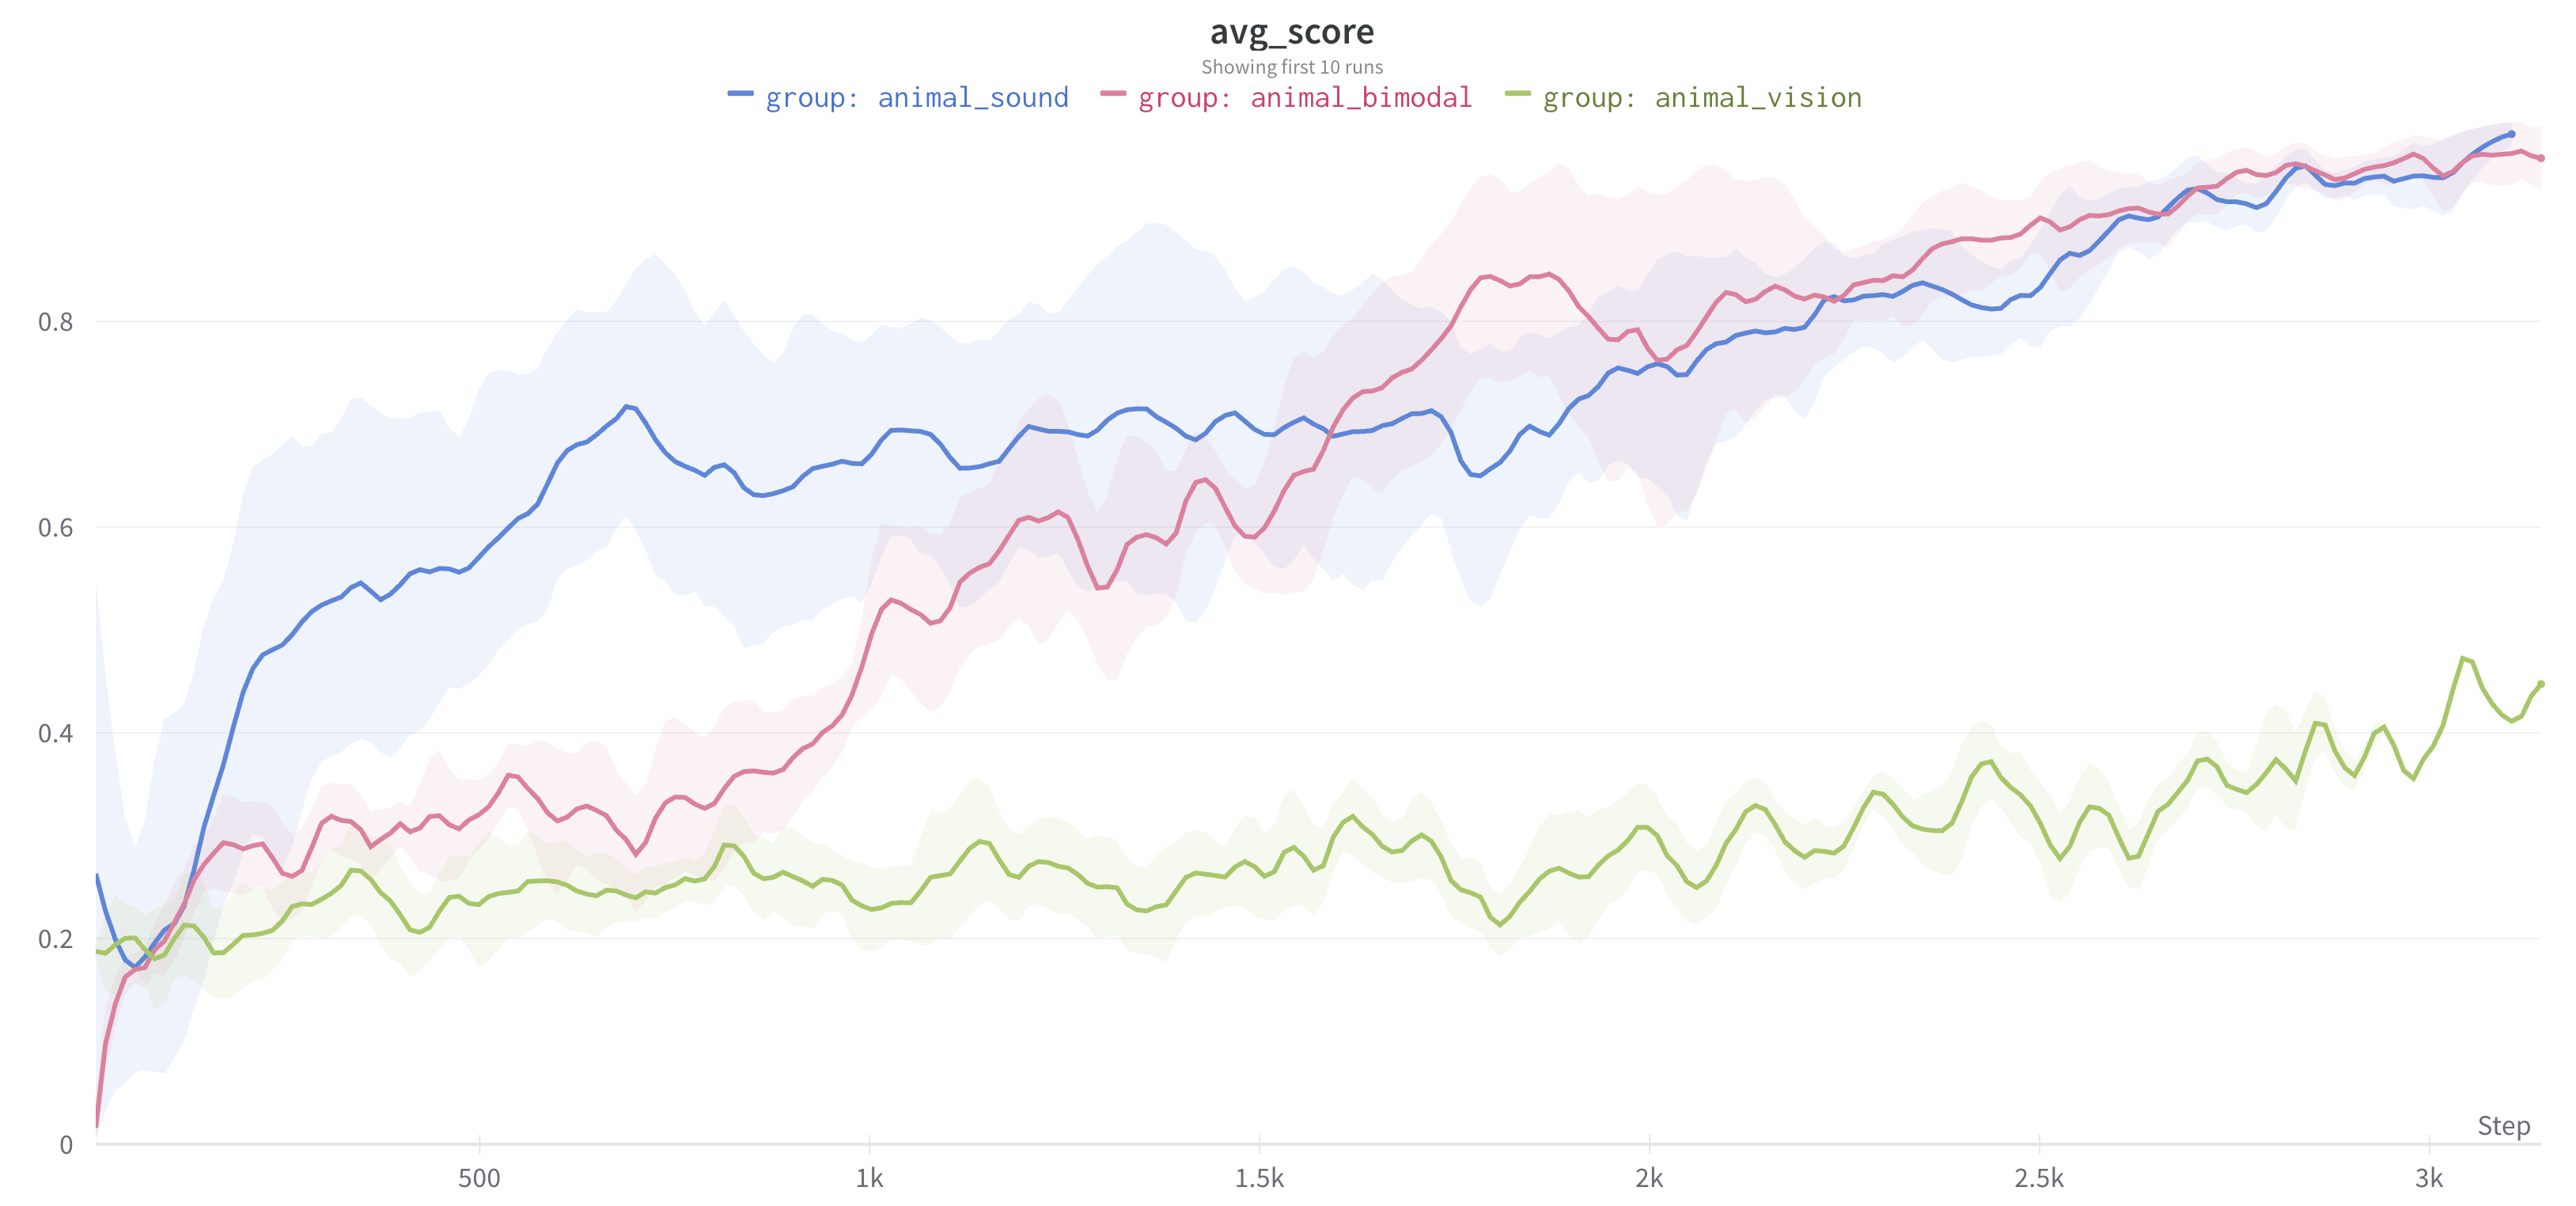
\includegraphics[width=\textwidth]{animal.png}
    \caption{동물 찾아가기 태스크(동물)에 대한 비전, 소리, 멀티모달 에이전트의 성능을 나타낸 그래프이다.}
    \label{fig:animal}
\end{figure}
그림 \ref{fig:animal}을 보면 보상이 희박하기 때문에 세 에이전트에서 학습이 오래 걸리는 것을 볼 수 있다. \lstinline{animal_vision}으로 나타낸 비전 에이전트는 주어진 시간 내에 동물을 찾아가는 것을 학습하지 못하였다. \lstinline{animal_sound}로 나타낸 소리 에이전트와 \lstinline{animal_multimodal}로 나타낸 멀티모달 에이전트는 주어진 시간 내에 학습을 완료하였다.

\begin{figure}[H]
    \centering
    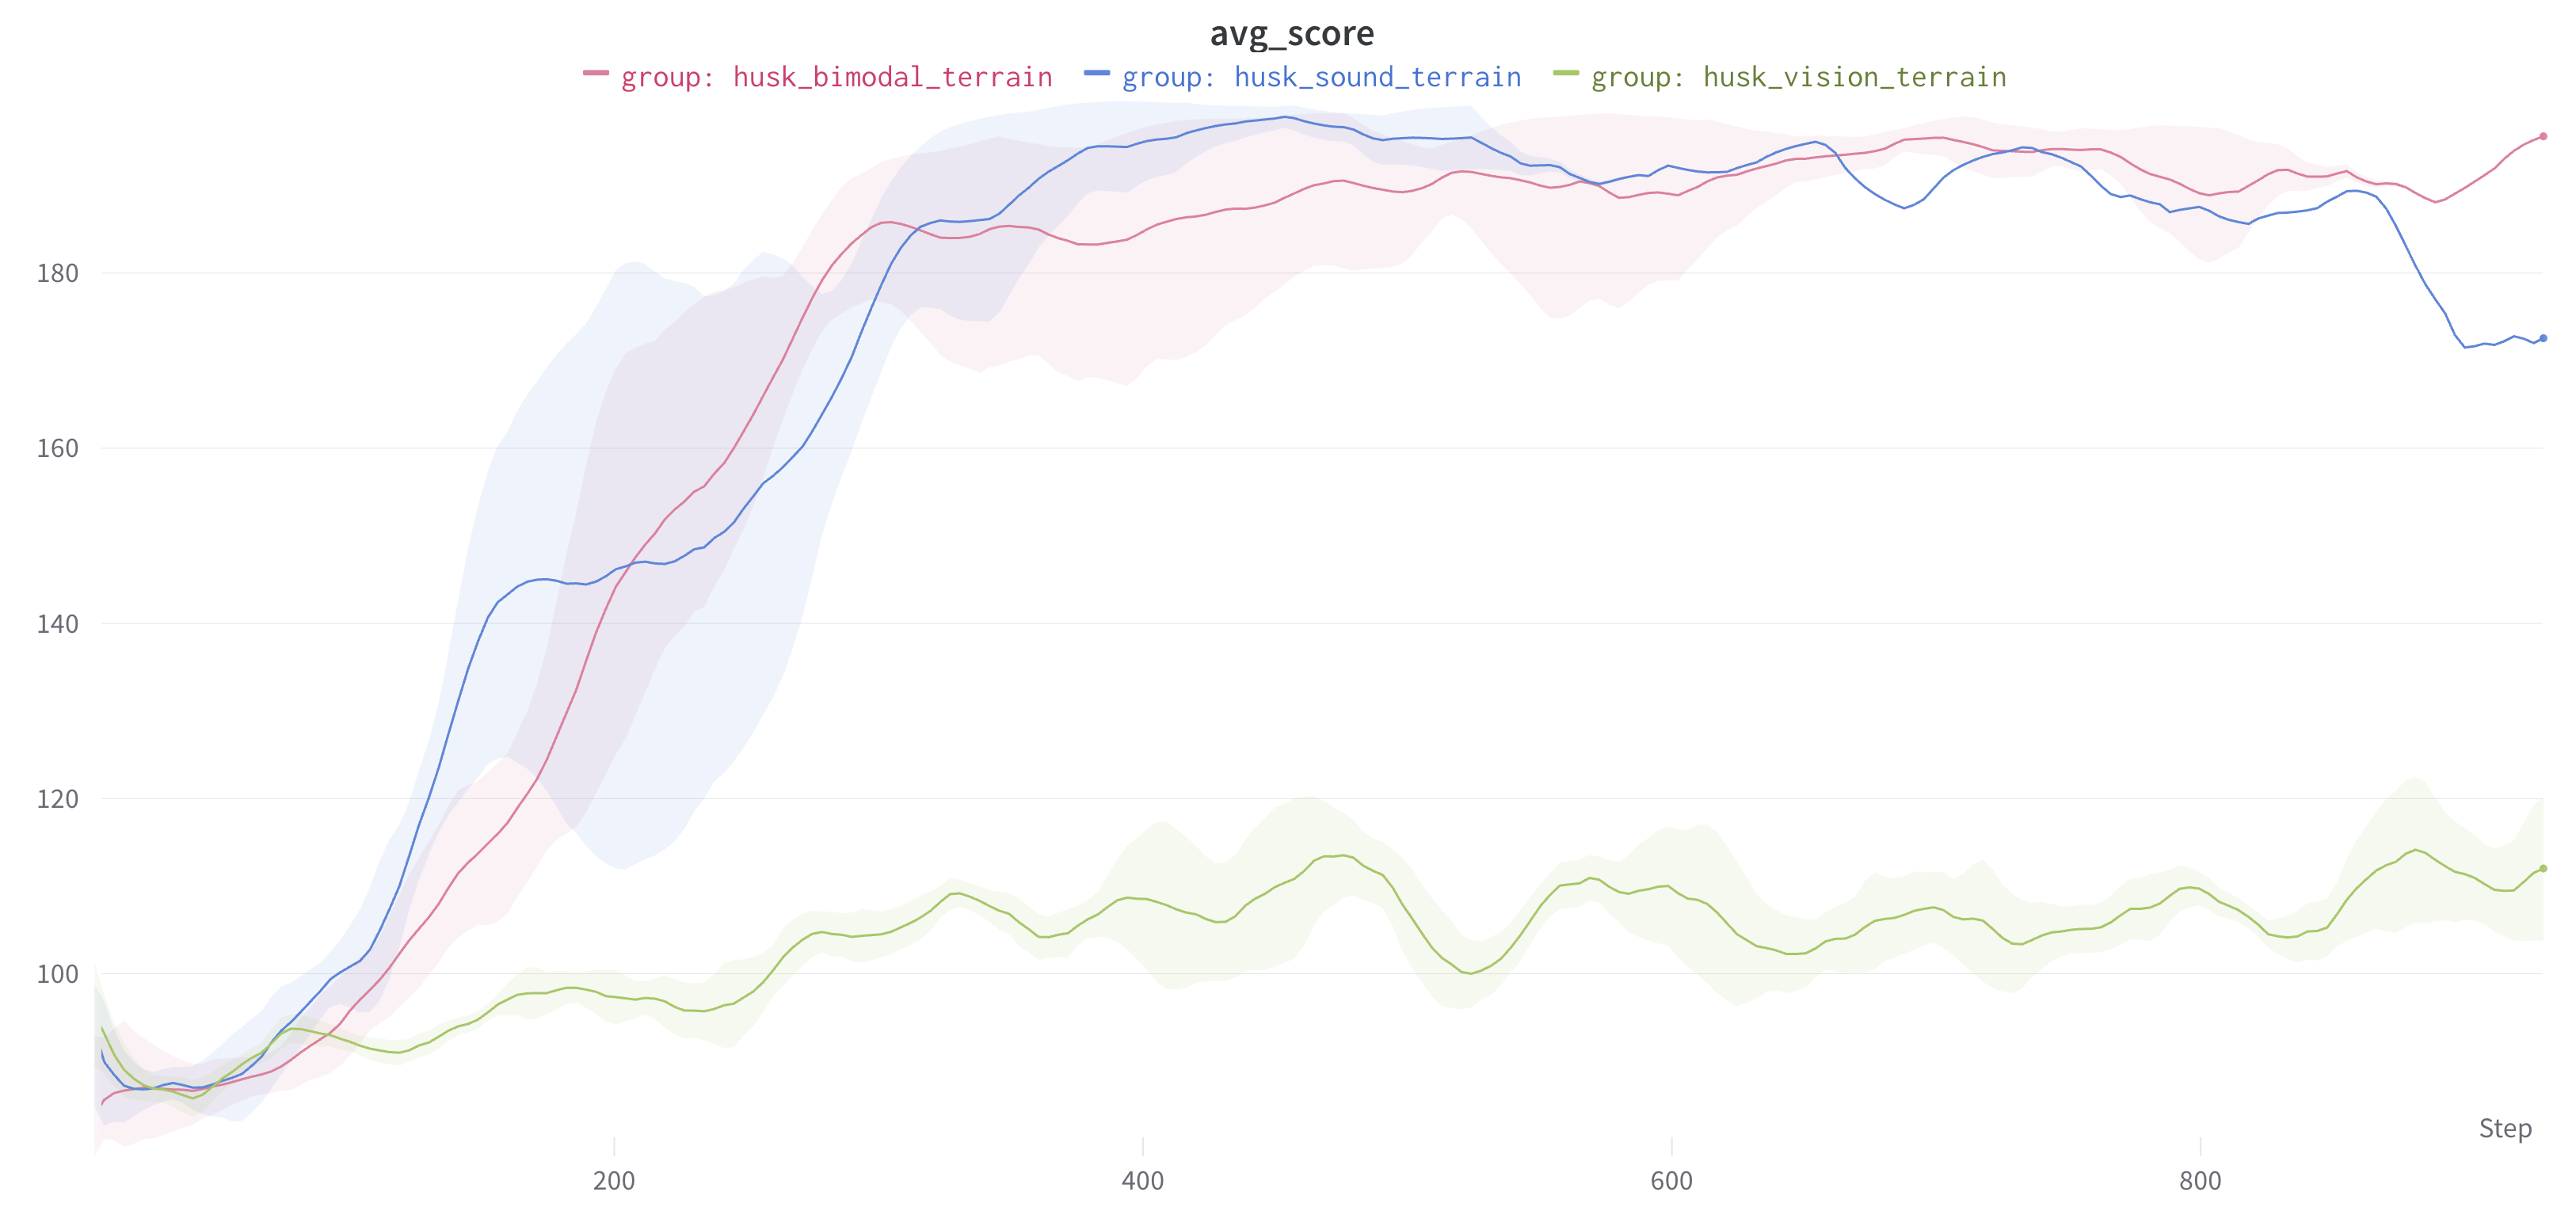
\includegraphics[width=\textwidth]{husk_terrain.png}
    \caption{장애물과 언덕이 있는 지형에서 허스크를 회피하는 태스크 (지형-허스크)에 대한 비전, 소리, 멀티모달 에이전트의 성능을 나타낸 그래프이다. }
    \label{fig:husk_terrain}
\end{figure}
그림 \ref{fig:husk_terrain}를 보면 \lstinline{husk_vision_terrain}으로 나타낸 비전 에이전트는 거의 상황에 대처하지 못하는 것을 볼 수 있으며, \lstinline{husk_sound_terrain}로 나타낸 소리 에이전트와 \lstinline{husk_multimodal_terrain}로 나타낸 멀티모달 에이전트는 장애물과 언덕이 있는 지형에서도 잘 대처하는 것을 확인할 수 있다.

이번 논문에서 이용한 4개의 환경에서, 비전만을 활용한 에이전트는 소리를 이용하는 에이전트나 소리와 비전을 모두 활용한 에이전트보다 성능이 현저히 낮은 것을 확인할 수 있었다. 이는 비전 정보가 해당 순간에 허스크를 효과적으로 피하거나 동물을 찾아가는 데에 충분한 정보를 제공하지 못하며, 신경망에 훈련해야 할 파라미터 수가 많아 주어진 훈련 횟수 내에 학습이 잘 이루어지지 못하기 때문이다. 반면 
소리만을 이용하는 에이전트의 경우 대부분의 태스크에서 최고의 성능을 보여주었다. 또한 소리만을 이용하는 에이전트의 경우 파라미터 수가 적어 더 빠른 시간 내에 학습이 진행되었다. 보상이 희박한 환경에서도 이 경향은 반전되지 않았다. 이는 소리 정보에는 자체적으로 소리의 방향과 거리, 종류에 대한 정보가 저차원 벡터에 저장되어 있어 특징을 추출하기 쉽기 때문이다. 언덕이 존재하는 지형에서의 허스크 피하기 태스크 (지형-허스크) 에서는 소리와 비전 모두를 이용하는 바이모달 에이전트의 성능이 가장 우수함을 확인할 수 있었다. 이는 소리를 내지 않는 장애물의 경우 소리에 의존하기보다는 비전 정보를 이용하여야 해당 장애물을 잘 피해갈 수 있기 때문이다. 종합적으로 비전만을 활용한 에이전트보다 소리 정보만, 또는 소리 정보를 추가적으로 이용한 에이전트의 성능이 더 우수한 것을 확인하였다.

\chapter{결론}\label{chp:conclusion}

마인크래프트를 기반으로 하는 강화학습 환경은 이미 존재하지만, 이들 환경에서는 대부분 비전 정보에 집중하며 게임 내에서 발생하는 소리에 대한 정보를 관측 공간으로써 제공하지 않는다. 이 연구에서는 기존 환경들이 제공하지 않던 소리라는 관측 공간 항목을 추가한 새로운 마인크래프트 기반 강화 학습 환경을 개발하였다. 이 환경을 이용하여 실험을 진행한 결과, 비전만을 이용하는 에이전트에 비해 소리를 이용하는 에이전트와 소리와 비전 모두를 활용하는 바이모달 에이전트의 성능이 더 우수함을 확인할 수 있었다. 또한 소리만을 이용하는 에이전트의 경우 빠른 시간 내에 학습이 완료되었다. 이는 이 연구에서 주어진 태스크에서 비전만을 이용하는 에이전트보다 소리 입력만 또는 소리와 비전을 모두 이용하는 에이전트가 더 효율적으로 학습할 수 있음을 보여준다. 이 연구를 통해 기존에 비전 정보에 비해 중요하게 여겨지지 않았던 소리 정보 내지 바이모달 정보를 이용하는 환경 및 강화학습 에이전트에 대한 관심을 제안한다.

앞으로의 연구 방향으로는 중요한 정보가 들어 있는(예측 Q 값과 실제 Q 값의 오차가 큰) 전이를 더 자주 추출하는 리플레이 버퍼 전략인 Prioritized Experience Replay \cite{per}나 순환 신경망을 이용하여 최근 N개의 관측을 활용하는 DRQN \cite{POMDP}, 호기심 기반 탐색 \cite{curious}과 같은 기술을 적용해 보는 것과 함께, Advantage Actor Critic \cite{A2C}이나 Proximal Policy Optimization \cite{PPO}과 같은 Policy Gradient 방법을 시도해 보는 것이다. 이를 통해 보다 정교한 강화 학습 알고리즘을 구축 및 실험하고, 우리의 시스템 성능을 더욱 향상시킬 수 있을 것으로 기대된다. 또한 이번 연구에서 알아낸 Q 값 기반 강화학습에 미치는 바이모달 에이전트의 성능과 policy gradient 방식 강화학습에 미치는 바이모달 에이전트의 성능에 대한 비교를 해볼 수 있을 것이다. 또한 이번 연구에서 활용한 환경들은 비교적 간단한 것들이었기에, 더 복잡한 환경에서 더 어려운 태스크를 수행하는 것도 시도해볼 수 있다. 이러한 연구는 인간의 감각체계와 유사한 기능을 가진 인공 시스템의 발전에 기여할 것이며, 다양한 실제 응용 분야에서 유용하게 활용될 수 있을 것이다.

%\appendix
%
%\chapter{My Appendix}
%\lipsum[1-3]
\bibliographystyle{ieeetr}
\begin{thebibliography}{00}

    \bibitem{minerl}Guss, W., Houghton, B., Topin, N., Wang, P., Codel, C., Veloso, M. \& Salakhutdinov, R. MineRL: A Large-Scale Dataset of Minecraft Demonstrations. {\em CoRR}. \textbf{abs/1907.13440} (2019), http://arxiv.org/abs/1907.13440

    \bibitem{minedojo}Fan, L., Wang, G., Jiang, Y., Mandlekar, A., Yang, Y., Zhu, H., Tang, A., Huang, D., Zhu, Y. \& Anandkumar, A. MineDojo: Building Open-Ended Embodied Agents with Internet-Scale Knowledge.  (2022)

    \bibitem{minedojoGithub}
    MineDojo. (2023). \textit{MineDojo GitHub Repository}. GitHub repository. Retrieved from \url{https://github.com/MineDojo/MineDojo/blob/main/minedojo/sim/Malmo/Minecraft/build.gradle#L70}

    \bibitem{POMDP}Hausknecht, M. \& Stone, P. Deep Recurrent Q-Learning for Partially Observable MDPs. {\em CoRR}. \textbf{abs/1507.06527} (2015), http://arxiv.org/abs/1507.06527

    \bibitem{DQN}Mnih, V., Kavukcuoglu, K., Silver, D., Graves, A., Antonoglou, I., Wierstra, D. \& Riedmiller, M. Playing Atari with Deep Reinforcement Learning. {\em CoRR}. \textbf{abs/1312.5602} (2013), http://arxiv.org/abs/1312.5602

    \bibitem{DuelingDQN}Wang, Z., Freitas, N. \& Lanctot, M. Dueling Network Architectures for Deep Reinforcement Learning. {\em CoRR}. \textbf{abs/1511.06581} (2015), http://arxiv.org/abs/1511.06581

    \bibitem{Rotation}Zhou, Y., Barnes, C., Lu, J., Yang, J. \& Li, H. On the Continuity of Rotation Representations in Neural Networks. {\em CoRR}. \textbf{abs/1812.07035} (2018), http://arxiv.org/abs/1812.07035

    \bibitem{gym}Brockman, G., Cheung, V., Pettersson, L., Schneider, J., Schulman, J., Tang, J. \& Zaremba, W. OpenAI Gym. {\em CoRR}. \textbf{abs/1606.01540} (2016), http://arxiv.org/abs/1606.01540

    \bibitem{per}Schaul, T., Quan, J., Antonoglou, I. \& Silver, D. Prioritized Experience Replay.  (2015), http://arxiv.org/abs/1511.05952, cite arxiv:1511.05952Comment: Published at ICLR 2016

    \bibitem{curious}Pathak, D., Agrawal, P., Efros, A. \& Darrell, T. Curiosity-driven Exploration by Self-supervised Prediction. {\em CoRR}. \textbf{abs/1705.05363} (2017), http://arxiv.org/abs/1705.05363


    \bibitem{A2C}Mnih, V., Badia, A., Mirza, M., Graves, A., Lillicrap, T., Harley, T., Silver, D. \& Kavukcuoglu, K. Asynchronous Methods for Deep Reinforcement Learning. {\em CoRR}. \textbf{abs/1602.01783} (2016), http://arxiv.org/abs/1602.01783

    \bibitem{PPO}Schulman, J., Wolski, F., Dhariwal, P., Radford, A. \& Klimov, O. Proximal Policy Optimization Algorithms. {\em CoRR}. \textbf{abs/1707.06347} (2017), http://arxiv.org/abs/1707.06347


\end{thebibliography}



% \bibliography{biblio}



\newpage
\keywordalt{Reinforcement Learning, Minecraft, Multimodal, Bimodal, Sound}
\addcontentsline{toc}{chapter}{\abstractnamealt}
\begin{center}
    \fontsize{16}{32}\selectfont
    \abstractnamealt\\
    \fontsize{22}{36}\selectfont
    The Utility of Various Modalities in Reinforcement Learning with Minecraft Learning Environment
    \vspace{1cm}
    \fontsize{14}{21}\selectfont
    \begin{flushright}
        Hyeonseo Yang\\
        Department of Computer Science and Engineering\\
        The Undergraduate School \\ 
        Seoul National University \\ 
    \end{flushright}
		
\end{center}

\begin{center}
    \fontsize{11}{16}\selectfont
    There already exist some reinforcement learning environments based on Minecraft. However, most of these environments primarily focus on visual information and do not provide observations for in-game sounds. Consequently, many reinforcement learning agents developed for such environments rely solely on visual inputs. In this research, we introduce a novel reinforcement learning environment called "mydojo" based on Minecraft. This environment incorporates a new observation space item, namely sound, which was not offered in existing environments. Using this addition, we implement agents that utilize sound as well as agents that leverage both sound and vision, and compare their performance with agents that solely rely on vision, which has been the predominant input modality in previous approaches. Through this comparison, we highlight the significance of sound information, which has been relatively overlooked compared to visual information, and emphasize the importance of multimodal processing. By evaluating the performance of these agents on tasks such as avoiding single or multiple husks that attack the Minecraft player and locating specific animals in a ranch environment, we observe that the agents utilizing the newly added sound observation space or both sound and vision significantly outperform the agents relying solely on vision. Moreover, these agents demonstrate shorter learning times. This research aims to garner attention towards the utilization of sound information and multimodal processing, which have been undervalued compared to vision, in both the design of Minecraft-based environments and reinforcement learning agents.
\end{center}

\vfill\vspace*{\fill}
	% better than "\vfill", "\null\vfill", \vspace*{0pt}\vfill", etc.
	\noindent
	{\bfseries \keywordnamealt}: Reinforcement Learning, Minecraft, Multimodal, Bimodal, Sound 

\end{document}
